\documentclass{report}
\usepackage{amsmath}
\usepackage{amssymb}
\usepackage{amsthm}
\usepackage{amscd}
\usepackage[usenames,dvipsnames,svgnames,table]{xcolor}
\usepackage[colorlinks=true,urlcolor=blue,bookmarks=true,citecolor=blue]{hyperref}
\usepackage{fullpage}
\usepackage{braket}
\usepackage{dsfont}
\usepackage{slashed}
\usepackage{comment}
\usepackage{verbatim}
\usepackage{mathrsfs}
\usepackage{mathtools}
\usepackage{tikz}
\usetikzlibrary{tqft}
\usetikzlibrary{positioning}
\usetikzlibrary{decorations}
\usetikzlibrary{decorations.markings}
\usetikzlibrary{decorations.pathmorphing}
\usetikzlibrary{shapes.misc,fit}

\theoremstyle{plain}
\newtheorem{theorem}{Theorem}[section]
\newtheorem{lemma}[theorem]{Lemma}
\newtheorem{proposition}[theorem]{Proposition}
\newtheorem{conjecture}[theorem]{Conjecture}
\newtheorem{corollary}[theorem]{Corollary}

\theoremstyle{definition}
\newtheorem{definition}[theorem]{Definition}
\newtheorem{axiom}{Axiom}
\newtheorem{example}[theorem]{Example}
\newtheorem{exercise}{Exercise}[section]

\theoremstyle{remark}
\newtheorem*{remark}{Remark}
\newtheorem*{note}{Note}

\newcommand{\FR}[2]{\frac{#1}{#2}}
\newcommand{\PFR}[2]{\left(\frac{#1}{#2}\right)}
\newcommand{\SFR}[2]{\sqrt{\frac{#1}{#2}}}

\newcommand{\mc}{\mathcal}
\newcommand{\ms}{\mathscr}
\newcommand{\lam}{\lambda}
\newcommand{\vphi}{\varphi}
\newcommand{\om}{\omega}
\newcommand{\Om}{\Omega}
\newcommand{\gam}{\gamma}
\newcommand{\sg}{\sigma}
\newcommand{\di}{\partial}
\newcommand{\sdi}{\slashed\partial}
\newcommand{\ddi}[2]{\FR{\partial {#1}}{\partial {#2}}}
\newcommand{\hp}{\hat p}
\newcommand{\ha} { a}
\newcommand{\hb} { b}
\newcommand{\hbd} { b^\dagger}
\newcommand{\had}{ a^\dagger}
\newcommand{\iden}{\mathds{1}}
\newcommand{\colr}[1]{ {\color{red} #1 } }
\newcommand{\colb}[1]{ {\color{blue} #1 } }
\newcommand{\colf}[1]{ {\color{Fuchsia} #1 } }
 % normal ordering
\newcommand{\NO}[1]{\vcentcolon\mathrel{#1}\vcentcolon\,}
% creation annihilation normal ordering
\newcommand{\circcolon}{\mathbin{\raise 0.75ex\hbox{\oalign{$\scriptscriptstyle\mathrm{o}$\cr$\scriptscriptstyle\mathrm{o}$}}}}
\newcommand{\CANO}[1]{\,\circcolon\mathrel{#1}\circcolon\,} 

\newcommand{\elaborate}{{\color{blue} \textbf{Elaborate.}}}
\newcommand{\CHECK}{{\color{blue} \textbf{CHECK}}}

\newcommand{\bC}{\mathbb{C}}
\newcommand{\bR}{\mathbb{R}}
\newcommand{\bP}{\mathbb{P}}
\newcommand{\bN}{\mathbb{N}}
\newcommand{\bZ}{\mathbb{Z}}
\newcommand{\bH}{\mathbb{H}}
\newcommand{\cA}{\mathcal{A}}
\newcommand{\cB}{\mathcal{B}}
\newcommand{\cC}{\mathcal{C}}
\newcommand{\cD}{\mathcal{D}}
\newcommand{\cF}{\mathcal{F}}
\newcommand{\cG}{\mathcal{G}}
\newcommand{\cH}{\mathcal{H}}
\newcommand{\cI}{\mathcal{I}}
\newcommand{\cJ}{\mathcal{J}}
\newcommand{\cL}{\mathcal{L}}
\newcommand{\cM}{\mathcal{M}}
\newcommand{\cP}{\mathcal{P}}
\newcommand{\cV}{\mathcal{V}}
\newcommand{\cX}{\mathcal{X}}
\newcommand{\fg}{\mathfrak{g}}
\newcommand{\fso}{\mathfrak{so}}
\newcommand{\diff}{\mathrm{diff}}
\newcommand{\Weyl}{\mathrm{Weyl}}
\newcommand{\detFP}{\Delta_{\text{FP}}}
\DeclareMathOperator{\id}{id}
\DeclareMathOperator{\Vol}{Vol}
\DeclareMathOperator{\End}{End}
\DeclareMathOperator{\Tot}{Tot}
\DeclareMathOperator{\diag}{diag}
\DeclareMathOperator{\im}{Im}
\DeclareMathOperator{\Sym}{Sym}
\DeclareMathOperator{\re}{Re}
\DeclareMathOperator{\Ad}{Ad}
\DeclareMathOperator{\Sp}{Sp}
\DeclareMathOperator{\PSL}{PSL}
\DeclareMathOperator{\SO}{SO}
\DeclareMathOperator{\vspan}{span}
\DeclareMathOperator{\Hom}{Hom}
\DeclareMathOperator{\Aut}{Aut}
\DeclareMathOperator{\Res}{Res}
\DeclareMathOperator{\Teich}{Teich}
\DeclareMathOperator{\Diff}{Diff}
\DeclareMathOperator{\Met}{Met}
\DeclareMathOperator{\Mod}{Mod}
\DeclareMathOperator{\Conf}{Conf}
\DeclareMathOperator{\CKG}{CKG}
\DeclareMathOperator{\Fixed}{Fixed}
\newcommand{\eff}{\text{eff}}
\newcommand{\vacuum}{\text{vacuum}}
\newcommand{\pp}{\text{pp}}
\newcommand{\dder}[2]{\frac{d #1}{d #2}}
\newcommand{\pder}[2]{\frac{\partial #1}{\partial #2}}
\newcommand{\fder}[2]{\frac{\delta #1}{\delta #2}}
\newcommand{\pdder}[2]{\frac{\partial^2 #1}{\partial #2^2}}
\newcommand{\bz}{\bar{z}}
\newcommand{\bu}{\bar{u}}
\newcommand{\bdi}{\bar{\di}}

\begingroup
    \makeatletter
    \@for\theoremstyle:=definition,remark,plain\do{%
        \expandafter\g@addto@macro\csname th@\theoremstyle\endcsname{%
            \addtolength\thm@preskip\parskip
            }%
        }
\endgroup

\edef\restoreparindent{\parindent=\the\parindent\relax}
\usepackage{parskip}
\restoreparindent

\tikzset{
  directed/.style={postaction=decorate,
    decoration={markings,mark=at position .5 with {\arrow{>}}}},
  fermion/.style={thick,draw=black},
  photon/.style={draw=black,decorate,decoration=snake},
  gluon/.style={draw=black,decorate,decoration={coil,aspect=0}},
  vertex/.style={shape=circle,scale=0.5,fill=black,draw=black},
  counterterm/.style={shape=circle,draw=black,
    append after command={node[draw=black,fit=(\tikzlastnode),
      inner sep=-7\pgflinewidth,cross out] {}}},
  interaction/.style={shape=circle,scale=2,fill=gray,draw=black},
  every loop/.style={thick,draw=black},
  loop left/.style={in=140,out=220,min distance=2cm},
  loop right/.style={in=-40,out=40,min distance=2cm},
  loop above/.style={in=60,out=120,min distance=2.4cm},
  loop below/.style={in=-120,out=-60,min distance=2.4cm}
}

\title{String Theory and Supersymmetry\\Winter 2016 Seminar Notes}
\author{Anton Borissov, Henry Liu}
\date{\today}

\begin{document}
\hypersetup{pageanchor=false}
\maketitle
\hypersetup{pageanchor=true}

\tableofcontents

\chapter{Introduction to Strings}

We asked ``why fields?'' when we started QFT; now we ask, why strings?
Here are some potentially convincing reasons.
\begin{enumerate}
\item If we allow one more degree of freedom than particles, many
  IR/UV divergences disappear; we require less renormalization. If we
  allow more than one degree of freedom, new divergences arise from
  the increased internal degrees of freedom.
\item Every consistent string theory contains a massless spin-$2$
  state, i.e. a graviton, whose interactions at low energies reduce to
  general relativity.
\item The Standard Model, based on QFT, has $25$ adjustable constants.
  String theory has none, and leads to gauge groups big enough to
  include the Standard Model.
\item Consistent string theories force upon us supersymmetry and
  extra dimensions, which have arisen naturally from several different
  attempts to unify the Standard Model.
\end{enumerate}

Regardless of whether they are convincing, we start in this chapter,
as with any other physical model, by writing down an action.
Specifically, we first write the action for a relativistic string by
generalizing that of a relativistic point particle, and then we
quantize the action. As with QFT there are different ways to quantize.
We go through the analogue of canonical quantization in order to
quickly compute the spectrum of a string, and then go through path
integral quantization in preparation for studying string interactions.

As usual, we take $\hbar = c = 1$, and use {\bf Einstein summation
  convention}: repeated indices are implicitly summed over.

\section{Review of Relativity}

We work in $\bR^{D-1,1}$ where $D$ is the {\bf number of dimensions}.
Recall that coordinates are written $x^\mu = (x^0, x^1, \ldots, x^D) =
(ct, x^1, \ldots, x^D)$, and the metric is
\[ -ds^2 \coloneqq \eta_{\mu\nu} dx^\mu dx^\nu, \quad \eta_{\mu\nu} = \diag(-1, 1, 1, \ldots, 1). \]
Note that $\eta^\mu{}_\mu = D$. We use the dot product to stand for
the {\bf Lorentz inner product}, e.g. $-ds^2 = dx \cdot dx$.

\begin{definition}
  Define the {\bf proper time} of a system as the time elapsed
  measured by a clock traveling in the same Lorentz frame as the
  system itself. In such a Lorentz frame, $dx^i = 0$ and $dt$ is the
  proper time elapsed, so $-ds^2 = -dt_p^2$; define
  \[ ds \coloneqq \sqrt{ds^2} = dt_p \qquad \text{whenever } ds^2 > 0, \]
  i.e. for timelike intervals. Hence $ds$ is the {\bf proper time
    interval}. The {\bf relativistic momentum} is $p^\mu \coloneqq
  m(dx^\mu/ds)$. Conveniently,
  \[ p^\mu p_\mu = m^2\dder{x^\mu}{s} \dder{x_\mu}{s} = -m^2 \dder{s^2}{s^2} = -m^2. \]
\end{definition}

\begin{definition}
  A {\bf Lorentz transformation} $\Lambda^\mu{}_\nu$ is an element of
  the Lorentz group, the collection of all linear isometries of
  $\bR^{D-1,1}$. We say $a^\mu$ is a {\bf vector} if under Lorentz
  transformations, it changes as $a'^\mu = \Lambda^\mu{}_\nu a^\nu$. A
  {\bf Poincar\'e transformation} is a Lorentz transformation possibly
  followed by a translation.
\end{definition}

\begin{definition}
  The {\bf world line} of a point particle is the path in spacetime
  $\bR^{D-1,1}$ traced out by the particle as it evolves in time.
\end{definition}

The underlying principle of relativity says that physical laws are
independent of Lorentz frame. In other words, any action we write down
that we want to be compatible with relativity must have external
symmetries: it must be invariant under Lorentz transformations. We
call this {\bf Lorentz invariance}. As long as superscripts and
subscripts match up, we do not have to worry about Lorentz invariance.

The {\bf action} for a free relativistic {\bf point particle} is
obtained by writing down the simplest Lorentz invariant action, and
then making sure dimensions work out. If $\gamma$ is the path taken by
the particle, the action is therefore
\[ S_{\pp}[x] \coloneqq -m\int_\gamma ds = -m\int_\gamma d\tau \, \sqrt{-\eta_{\mu\nu} \dder{x^\mu}{\tau} \dder{x^\nu}{\tau}} = -m\int_\gamma d\tau \, \sqrt{-\dot{x}^\mu \cdot \dot{x}_\mu} \]
where a dot denotes a $\tau$-derivative. Because $ds$ is
coordinate-independent, it does not what how we pick the
parametrization $\tau$. Physicists like to call this {\bf
  reparametrization invariance}. This invariance is very important:
without it, we have actually introduced a completely new parameter
$\tau$, thus increasing the number of degrees of freedom from $D-1$ to
$D$.

\begin{exercise}
  By computing $\delta(ds^2)$ in two different ways, show that
  \[ \delta S_{\pp}[x] = m\int_\gamma \delta(dx^\mu) \frac{dx_\mu}{ds} = \int_\gamma d\tau \left(\dder{}{\tau} \delta x^\mu\right) p_\mu = \delta x^\mu p_\mu\bigg|_{\tau_i}^{\tau_f} - \int d\tau \delta x^\mu \dder{p_\mu}{\tau}. \]
  Argue that the first term vanishes if we specify {\bf initial and
    final conditions}. Hence deduce the equation of motion
  $dp_\mu/d\tau = 0$.
\end{exercise}

The action $S_{\pp}$ seems simple in the $\int_\gamma ds$ form, but is
messy when parametrized. Later when we quantize using path integrals,
$S_{\pp}$ is difficult to work with because of the derivatives under
the square root. There is a different, classically-equivalent action
we can work with. Introduce an additional field
$\gamma_{\tau\tau}(\tau)$ (sometimes called an {\bf einbein} in
general relativity), which we can view as a metric on the world line,
and take the action
\[ S'_{\pp} \coloneqq -\frac{1}{2} \int_\gamma d\tau \sqrt{-\gamma_{\tau\tau}} (\gamma^{\tau\tau} \dot{x}^\mu \dot{x}_\mu + m^2) = -\frac{1}{2} \int_\gamma d\tau \, (\eta^{-1} \dot{x}^\mu \dot{x}_\mu - \eta m^2), \quad \eta \coloneqq \sqrt{-\gamma_{\tau\tau}(\tau)}. \]
It seems like we have arbitrarily added an extra degree of freedom,
but in fact $\gamma$ is completely specified by the equation of
motion. The action $S'_{\pp}$ is much better to work with in a path
integral, because it is {\bf quadratic} in $\dot{x}^\mu$.

\begin{exercise}
  Vary $S'_{\pp}$ with respect to $\gamma_{\tau\tau}$ to get the
  equation of motion $\gamma_{\tau\tau} = \dot{x}^\mu
  \dot{x}_\mu/m^2$. Substitute this expression back into $S'_{\pp}$ to
  obtain $S_{\pp}$, and therefore conclude that the two actions are
  classically equivalent.
\end{exercise}

\section{Nambu--Goto and Polyakov Actions}

We graduate to {\bf one-dimensional strings}; in this section we write
down an action for them. There are two kinds of strings: those with
two distinct endpoints, called {\bf open strings}, and those which are
loops, called {\bf closed strings}. Because closed strings are just
open strings with the extra constraint that the two endpoints match,
we focus on open strings.

The action for the relativistic point particle is proportional to the
proper time elapsed on the particle's world line. But the proper time,
when multiplied by $c$, can be viewed as the ``proper length'' of the
world line. The natural generalization, then, is to consider the
surface in space-time traced out by the string as it evolves in time,
called the {\bf world sheet} $\Sigma$, and to define an action
proportional to the ``proper area'' of the world sheet. The world
sheet $\Sigma$ is a two-dimensional surface, and therefore requires
charts modeled on $\bR^2$.

\begin{definition}
  The {\bf coordinates} we use on $\bR^2$, the parameter space, are
  denoted $(\sigma^0, \sigma^1)$, and so the {\bf world sheet}
  $\Sigma$ is locally a surface given by functions denoted
  $X^\mu(\sigma)$ (capitalized to disambiguate from the coordinates
  $x^\mu$), called {\bf string coordinates}. The lowercase Latin
  characters $a, b, \ldots$ are used to denote {\bf indices} that run
  over values $0,1$. Two notes:
  \begin{enumerate}
  \item The choice of parametrization $(\sigma^0, \sigma^1)$ is,
    again, up to us, but usually we take the coordinate $\sigma^0$ to
    be the proper time, and $\sigma^1$ the position along the string.
  \item For our purposes, $\Sigma = X^\mu$, i.e. the single chart
    $X^\mu$ describes the entire world sheet for the region of
    spacetime we care about.
  \end{enumerate}
\end{definition}

\begin{exercise}
  Show that the metric $\eta_{\mu\nu}$ on spacetime $\bR^{D-1,1}$
  induces a metric $g$ on the world sheet via pullback along the
  inclusion $\iota\colon \Sigma \to \bR^{D-1,1}$. Compute $g$ and the
  area element:
  \[ g_{ab} = \di_a X^\mu \di_b X_\mu, \quad dA =  d^2\sigma \, \sqrt{-\det g}. \]
\end{exercise}

A relativistic particle has a parameter we call mass. It turns out
mass is not the appropriate physical interpretation of the
corresponding parameter for strings. Instead, we interpret it as a
{\bf tension}, and denote it $T_0$. Old people write $T_0 = 1/2\pi
\alpha'$ and call $\alpha'$ the {\bf universal Regge slope}; we choose
not to.

\begin{definition}
  The {\bf Nambu--Goto action} for a relativistic string is given by
  \[ S_{\text{NG}}[X] \coloneqq -T_0 \int_\Sigma dA = -T_0 \int_\Sigma d^2\sigma \, \sqrt{-\det g}. \]
  Again, note that it satisfies {\bf reparametrization invariance},
  literally by construction.
\end{definition}

But again, we have a square root and derivatives inside it, and now we
know how to get rid of it: introduce an independent world sheet metric
$\gamma_{ab}(\sigma)$. This time the metric is on a surface, so
we need to specify the signature. We take Lorentzian signature $(-,
+)$.

\begin{definition}
  The {\bf Polyakov action} for a relativistic string is given by
  \[ S_{\text{P}}[X, \gamma] \coloneqq -\frac{T_0}{2} \int_\Sigma d^2\sigma \, \sqrt{-\gamma} \, \gamma^{ab} \di_a X^\mu \di_b X_\mu, \]
  where $\gamma$ without indices stands for $\det(\gamma_{ab})$. From
  now on, we always refer to $\gamma_{ab}$ as the {\bf metric}, and
  $g_{ab}$ as the {\bf induced metric}. World sheet indices are
  raised/lowered using the metric $\gamma_{ab}$, not the induced
  metric $g_{ab}$. (In fact, from now on we basically forget about
  $g_{ab}$; we use it only to introduce the Nambu--Goto action, and
  the following exercise.)
\end{definition}

\begin{exercise}
  Show that $\delta \sqrt{-\gamma} = (1/2)\sqrt{-\gamma} \,
  \gamma^{ab} \delta \gamma_{ab}$, and therefore that
  \[ \delta_\gamma S_{\text{P}}[X, \gamma] = -\frac{T_0}{2} \int_\Sigma d^2\sigma \, \sqrt{-\gamma} \, \delta \gamma^{ab} \left(g_{ab} - \frac{1}{2} \gamma_{ab} \gamma^{cd} g_{cd}\right). \]
  Rearrange the obtained equation of motion and conclude that
  $g_{ab}\sqrt{-g} = \gamma_{ab}\sqrt{-\gamma}$. Hence replace
  $\gamma$ in $S_{\text{P}}[X, \gamma]$ with $g$, and obtain that
  $S_{\text{P}}[X, \gamma] = S_{\text{NG}}[X]$.
\end{exercise}

\begin{definition}
  As in general relativity, define the {\bf stress-energy tensor}
  \begin{align}
      \label{stressenergydefn}
      T_{ab}(\sigma) \coloneqq -\frac{4\pi}{\sqrt{-\gamma}} \delta_{\gamma}
      S_{\text{P}}[X, \gamma] = -2\pi T_0 \left(\di_a X^\mu \di_b X_\mu -
      \frac{1}{2} \gamma_{ab} \di_c X^\mu \di^c X_\mu\right),\end{align}
  so that the equation of motion arising from varying $\gamma$ says
  $T_{ab} = 0$. We call $T_{ab} = 0$ a {\bf constraint} on the
  equation of motion for $X^\mu$, which we derive soon.
\end{definition}

\begin{exercise} (Important!)
  Now vary $S_{\text{P}}[X, \gamma]$ with respect to $X^\mu$ to obtain
  \begin{align*}
    \delta_X S_{\text{P}}[X, \gamma]
    &= -T_0 \int_\Sigma d^2\sigma \, \sqrt{-\gamma} \, \gamma^{ab} \left(\di_a(\delta X^\mu \di_b X_\mu) - \di_a \di_b X_\mu \delta X^\mu\right) \\
    &= -T_0 \int_0^{\ell} d\sigma^1 \, \sqrt{-\gamma} \left[\delta X^\mu \di^0 X_\mu\right]_{\sigma^0=\tau_i}^{\sigma^0=\tau_f} - T_0 \int_{\tau_i}^{\tau_f} d\sigma^0 \, \sqrt{-\gamma} \left[\delta X^\mu \di^1 X_\mu\right]_{\sigma^1=0}^{\sigma^1=\ell} \\
    &\qquad + T_0 \int_\Sigma d^2\sigma \, \sqrt{-\gamma} \, \delta X^\mu \nabla^2 X_\mu.
  \end{align*}
\end{exercise}

A careful inspection of the terms in the variation $\delta_X
S_{\text{P}}[X, \gamma]$ yield interesting insights. For this
variation to vanish, each of the terms must vanish independently,
since they control different aspects of the string's behavior.
\begin{enumerate}
\item The last term is determined by the motion of the string in the
  domain $(0, \ell) \times (\tau_i, \tau_f)$, and therefore $\delta
  X^\mu$ is not constrained by any boundary conditions there. Hence we
  have the {\bf equation of motion} $\sqrt{-\gamma} \, \nabla^2 X_\mu
  = 0$.
\item The first term is determined by the configuration of the string
  at times $\tau_i$ and $\tau_f$. If we specify these configurations
  as {\bf initial and final conditions}, then $\delta X^\mu$ is zero
  for the first term, so the term vanishes.
\item The second term is determined by the configuration of the
  endpoints of the string when $\sigma^0 \in (\tau_i, \tau_f)$. It
  does not vanish automatically. We have to impose {\bf boundary
    conditions} in order to make it vanish.
\end{enumerate}

\begin{definition}
  There are two different kinds of boundary conditions.
  \begin{itemize}
  \item The {\bf free (Neumann) boundary condition} is $\di^1
    X_\mu(\sigma^0, 0) = \di^1 X_\mu(\sigma^0, \ell) = 0$.
  \item The {\bf Dirichlet boundary condition} is $\delta
    X^\mu(\sigma^0, 0) = \delta X^\mu(\sigma^0, \ell) = 0$.
  \end{itemize}
  Alternatively, if the string is {\bf closed}, i.e. we have the {\bf
    periodicity} conditions
  \[ X^\mu(\sigma^0, 0) = X^\mu(\sigma^0, \ell), \quad \di^a X^\mu(\sigma^0, 0) = \di^a X^\mu(\sigma^0, \ell), \quad \gamma_{ab}(\sigma^0, 0) = \gamma_{ab}(\sigma^0, \ell), \]
  no additional boundary conditions are necessary.
\end{definition}

For a long time, string theorists did not seriously consider the
Dirichlet boundary condition. Why should the endpoints of an open
string be fixed, and if they were, where would they be fixed onto? In
particular, this fixing of endpoints would violate momentum
conservation. Then Polchinski, in the 1990s, suggested that the
endpoints are attached to {\bf D-branes}, which should themselves be
thought of as dynamical objects alongside strings. Conceptually, then,
\begin{enumerate}
\item a D$0$-brane is a particle, a D$1$-brane is a string, and so on,
  and they interact non-trivially;
\item the Dirichlet boundary condition says that a given D$1$-brane
  has fixed endpoints on a higher D$p$-brane;
\item any momentum lost by the D$1$-brane is absorbed by the
  D$p$-brane; and
\item the Neumann boundary condition is just saying there is a
  D-dimensional D-brane permeating all of space-time, i.e. the string
  endpoints are not fixed at all.
\end{enumerate}
We return to this D-brane perspective much later on. It is hard enough
to quantize strings without more dynamical objects floating around. We
take {\bf Neumann boundary conditions} for now.

\section{Gauge Freedom and Gauge Fixing}

There is another reason the Polyakov action is preferable over the
Nambu--Goto action: it has more symmetries, and these symmetries make
it easier to gauge fix (using Faddeev--Popov or otherwise) when we try
to quantize. The Polyakov action is invariant under the following
symmetries:
\begin{enumerate}
\item $D$-dimensional {\bf Poincar\'e transformations}:
  \[ X^\mu(\sigma) \mapsto \Lambda^\mu{}_\nu X^\nu(\sigma) + a^\mu, \quad \gamma_{ab}(\sigma) \mapsto \gamma_{ab}(\sigma); \]
\item {\bf Reparametrization} (i.e. diffeomorphisms): for new
  coordinates $\tilde{\sigma}^a(\sigma)$,
  \[ X^\mu(\sigma) \mapsto X^\mu(\tilde{\sigma}), \quad \gamma_{ab}(\sigma) \mapsto \pder{\sigma^c}{\tilde{\sigma}^a} \pder{\sigma^d}{\tilde{\sigma}^b} \gamma_{cd}(\sigma); \]
\item $2$-dimensional {\bf Weyl transformations}: for arbitrary
  $\omega(\sigma)$,
  \[ X^\mu(\sigma) \mapsto X^\mu(\sigma), \quad \gamma_{ab}(\sigma) \mapsto \exp(2\omega(\sigma)) \gamma_{ab}(\sigma). \]
  The Nambu--Goto action is not invariant under Weyl transformations.
\end{enumerate}

\begin{exercise}
  Verify all these statements. (This should be quite straightforward.)
\end{exercise}

\begin{definition}
  Let $\diff$ denote the group of diffeomorphisms acting on $\Sigma$,
  and $\Weyl$ the group of Weyl transformations acting on $\Sigma$;
  these are {\bf internal symmetries}, while Poincar\'e
  transformations are {\bf external symmetries}. The product $\diff
  \times \Weyl$ is the {\bf gauge group}. The orbit, in the space of
  all possible fields and metrics, of a particular $(X, \gamma)$ under
  the action of the gauge group is the {\bf gauge orbit}.
\end{definition}

A good exercise in working with the gauge and external symmetries is
to make sure Polyakov action is as general as possible. This also
reduces future work when we need the additional terms in the Polyakov
action. Note that here, contrary to the case in QFT, the symmetries
are very demanding. Weyl invariance in particular is very odd: it
prevents us from adding terms such as
\[ \int_\Sigma d^2\sigma \, \sqrt{-\gamma} \, V(X), \quad \mu \int_\Sigma d^2\sigma \, \sqrt{-\gamma}. \]

\begin{exercise}
  Convince yourself that the action must contain one more
  $\gamma^{ab}$ than $\gamma_{ab}$ in order to satisfy Weyl invariance
  and counteract the change in $\sqrt{-\gamma}$. Since such a
  $\gamma^{ab}$ can only pair up indices with derivatives, we need a
  second-order Lorentz-invariant term that is coordinate-independent.
  Convince yourself that other than $\di_a X^\mu \di_b X_\mu$, this
  term can only involve $\gamma^{ab}$ and $\gamma_{ab}$, and that in
  fact it must be the {\bf scalar curvature} $R$. Show that under a
  Weyl transformation,
  \[ \sqrt{-\gamma} \, R \mapsto \sqrt{-\gamma} (R - 2\nabla^2 \omega). \]
  Hence argue that we need another term integrated over $\di \Sigma$ to
  counteract $\nabla^2(\sqrt{-\gamma} \, \omega)$. Putting everything
  together, conclude that
  \[ \chi \coloneqq \frac{1}{4\pi} \int_\Sigma d^2\sigma \, \sqrt{-\gamma} \, R + \frac{1}{2\pi} \int_{\di \Sigma} ds \, k \]
  is Weyl invariant, and that it is essentially the only term we can
  add to the Polyakov action. Here $ds$ is proper time along $\di
  \Sigma$ using the metric $\gamma_{ab}$, and $k \coloneqq \pm t^a n_b
  \nabla_a t^b$ is the {\bf geodesic curvature} of the boundary, where
  $t^a$ is a unit vector tangent to the boundary, and $n_b$ an
  outward-pointing unit vector, and we choose $\pm$ depending on
  whether the boundary is timelike or spacelike.
\end{exercise}

Let's explore a few choices of gauge, some which use up all the gauge
freedom, and some which do not. We commonly use reparametrization
invariance to simplify expressions, so let's explore some choices of
gauge using reparametrization invariance first.

\begin{definition}
  We can reparametrize $(\sigma^0, \sigma^1)$ such that $\sigma^0$
  corresponds to the time coordinate $x^0$, i.e. $X^0 = R\sigma^0$ for
  some dimensionful constant $R$. This is {\bf static gauge}, named as
  such because then lines of constant $\sigma^0$ correspond to the
  string at fixed moments in time, i.e. the string is static. Another
  choice is {\bf light cone gauge}, given by $X^+ = R\sigma^0$, where
  \[ X^\pm \coloneqq \frac{1}{\sqrt{2}}(X^0 \pm X^1), \quad \sigma^\pm \coloneqq \frac{1}{\sqrt{2}}(\sigma^0 \pm \sigma^1) \]
  are {\bf light cone coordinates} on Minkowski space and the world
  sheet respectively. When in light cone gauge, the indices $i, j,
  \ldots$ range over $\{2, \ldots, D\}$.
\end{definition}

Clearly neither static gauge nor light cone gauge exhausts the gauge
freedom: we haven't done anything with the metric! But it is hard to
transform the metric in a useful way while staying in static or
light cone gauge. Let's take a different approach and try to transform
the metric first.

The transformation of the scalar curvature computed in the exercise
above says we can use Weyl invariance to locally set the scalar
curvature to zero, by solving $2\nabla^2\omega = R$ and then applying
the Weyl transformation $\exp(2\omega)$. But we are in two dimensions,
where the symmetries of the Riemann curvature tensor determine it from
$R$:
\[ R_{abcd} = R_{cdab}, \; R_{abcd} = -R_{bacd} = -R_{abdc} \implies R_{abcd} = (1/2)(\gamma_{ac}\gamma_{bd} - \gamma_{ad}\gamma_{bc}) R. \]
Hence we can always locally get a flat metric, which, possibly after
applying a coordinate transformation, gives $\gamma_{ab} = \eta_{ab}$,
the flat Minkowski metric.

\begin{definition}
  If we consider only reparametrization and not Weyl transformations,
  the metric $\gamma_{ab}$ can always be brought to the form
  $\exp(2\omega)\eta_{ab}$. Forcing the metric to be of that form is
  known as {\bf conformal gauge}. Performing the additional Weyl
  transformation to obtain $\gamma_{ab} = \eta_{ab}$ is known as {\bf
    unit gauge}. In general, the form of the metric we choose to put
  $\gamma_{ab}$ in is called the {\bf fiducial metric}.
\end{definition}

\begin{exercise} (Important!)
  Show that in unit gauge, the equation of motion and its
  constraints become
  \[ \di_a \di^a \vec{X} = 0, \quad \di_0\vec{X} \cdot \di_1\vec{X} = 0, \quad (\di_0\vec{X})^2 + (\di_1\vec{X})^2 = R^2. \]
  In this form, the constraints are called {\bf Virasoro conditions}.
  Argue that by tensoriality, the Virasoro conditions still hold in
  static gauge, where $X^\mu = (R\sigma^0, \vec{X})$. Hence show in
  static gauge that at the (free) endpoints an open string, i.e.
  endpoints satisfying the Neumann boundary condition, $|\di_t\vec{X}|
  = 1$. ({\bf Be careful}: $\di_t$ is not $\di_0$. What is $\di_t$?)
  Conclude that string endpoints always move at the speed of light.
\end{exercise}

How many internal degrees of freedom have we used up if we put the
metric $\gamma_{ab}$ in unit gauge? Well, $\diff$ has two degrees of
freedom, one for each coordinate, and $\Weyl$ has one, for the scale
of the metric. But the metric itself has three independent components,
being symmetric. Hence we expect to be done with choosing a
representative of each gauge orbit.

But, perhaps unexpectedly, there is more gauge freedom: there are
non-trivial transformations in $\diff \times \Weyl$ that preserve unit
gauge! The key to finding these transformations is to realize that
$\Sigma$ is actually a {\bf Riemann surface}: let $z \coloneqq
\sigma^0 + i\sigma^1$, so that $ds^2 = dz d\bar{z}$. Now if $f(z)$ is
a holomorphic change of coordinates, then
\[ z \mapsto f(z), \quad ds^2 \mapsto |\di_z f|^{-2} dz d\bar{z}, \]
so now applying the Weyl transformation $\exp(2 \ln |\di_z f|)$
recovers $ds^2$. Clearly the composition of the two transformations is
non-trivial.

What went wrong? Well, just because dimensions match up does not mean
we have spanned the whole space of gauge transformations! The
holomorphic diffeomorphisms above actually have {\bf measure zero} in
$\diff$. When we stop working locally and work globally instead, these
extra bits of freedom are removed by boundary conditions.

\begin{definition}
  When we successfully pick a unique and continuously-varying choice
  of representative in each gauge orbit, our theory is {\bf
    gauge-fixed}. When such a choice is impossible due to topological
  obstructions, our theory has {\bf Gribov ambiguity}. (For us, there
  is no Gribov ambiguity; we are just failing to consider boundary
  conditions.)
\end{definition}

\section{Quantization via Canonical Commutation Relations}

When we did QFT, we started by {\bf canonically quantizing} the
Klein-Gordon and Dirac fields, which allowed us to immediately
investigate some aspects of the quantized free theories, such as that
Klein-Gordon fields represent bosons and Dirac fields represent
fermions, and to obtain the spectrum and Hilbert space of states. On
the other hand, {\bf path integral quantization} gave us an easy way
to compute interactions in perturbative QFT, such as scattering
amplitudes. We do the same for string theory: first, in this section,
we canonically quantize in order to write down the spectrum and
Hilbert space of states, and then, in the next section, we quantize
using the path integral to work with interactions.

In string theory, canonical quantization no different from what we saw
in QFT. The procedure is the same: take the classical object (e.g.
Lagrangian, Hamiltonian, solutions) you want to quantize, and impose
{\bf canonical commutation relations} modeled on $[x, p] = i$ on
dynamical variables, by promoting them all to operators.

\subsection{Classical Solutions}

We take classical solutions and quantize them in light cone gauge as
well as two more gauge-fixing conditions for the metric: set
\[ X^+ = \sigma^0, \quad \di_1 \gamma_{11} = 0, \quad \det \gamma_{ab} = -1. \]
Note that we have dispensed with the dimensionful constant $R$; it can
be reinserted via dimensional analysis. The first thing to do right
after picking a gauge is to rewrite all the relevant objects in that
gauge. To do so, we need some formulas.

\begin{exercise}
  Show that in this gauge, $\gamma_{11}(\sigma^0)$ depends only on
  $\sigma^0$, and we have
  \[ \begin{pmatrix} \gamma^{00} & \gamma^{01} \\ \gamma^{10} & \gamma^{11} \end{pmatrix} = \begin{pmatrix} -\gamma_{11}(\sigma^0) & \gamma_{01}(\sigma) \\ \gamma_{01}(\sigma) & \gamma_{11}^{-1}(\sigma^0)(1 - \gamma_{01}^2(\sigma)) \end{pmatrix}. \]
  Furthermore, show that $\di_a X^\mu \di_a X_\mu = 2\di_a X^+ \di_a
  X^- - \di_a X^i \di_a X^i$. (Recall that indices $i, j, \ldots$
  range over $\{2, \ldots, D\}$).
\end{exercise}

\begin{definition}
  Given a dynamical variable $V(\sigma)$, define its associated {\bf
    center of mass} (conceptually at a fixed time) variables
  \[ v(\sigma^0) = \frac{1}{\ell} \int_0^\ell d\sigma^1 \, V(\sigma), \quad \tilde{V}(\sigma) = V(\sigma) - v(\sigma^0), \]
  i.e. we split $V = v + \tilde{V}$ where $v$ is the mean value of
  $V$, and $\tilde{V}$ has mean zero.
\end{definition}

For example, using that $\di_1X^+ = 0$, we have
\[ \di_1\tilde{X}^- = \di_1X^- = \frac{1}{\sqrt{2}}(\di_1X^0 - \di_1X^1) = \sqrt{2} \di_1X^0, \]
and using that $\di_0X^+ = 1$, we have
\[ \di_0X^0\di_1X^0 - \di_0X^1\di_1X^1 = (\di_0X^0 + \di_0X^1)\di_1X^0 - \di_0X^1(\di_1X^0 + \di_1X^1) = \sqrt{2} \di_1X^0 - 0. \]

\begin{exercise}
  Using all these calculations, show that the Polyakov Lagrangian in
  this gauge is
  \[ L = -\frac{T_0}{2} \int_0^\ell d\sigma^1 \bigg[\gamma_{11}(2\di_0X^- - \di_0X^i\di_0X^i) - 2\gamma_{01}(\di_1\tilde{X}^- - \di_0X^i \di_1X^i) + \gamma_{11}^{-1}(1 - \gamma_{01}^2) \di_1X^i \di_1X^i\bigg]. \]
  Argue that because $\tilde{X}^-$ does not appear with time
  derivatives, it is not a dynamical variable, and therefore when we
  vary $S_{\text{P}}$ with respect to $\gamma$, it constrains
  $\di_1\gamma_{01}$ to be zero. Show that the Neumann boundary
  condition, in this gauge, gives $\gamma_{01} = 0$ at the endpoints
  $\sigma = 0, \ell$, and conclude that $\gamma_{01} = 0$ everywhere.
  Therefore write down the simplified {\bf Lagrangian}:
  \[ L = -T_0\ell \gamma_{11}\di_0 x^- + \frac{T_0}{2} \int_0^\ell d\sigma^1 \, \left(\gamma_{11} \di_0X^i \di_0X^i - \gamma_{11}^{-1} \di_1X^i \di_1X^i\right), \]
\end{exercise}

The next step is to write down the Hamiltonian, which is the {\bf
  Legendre transform} of the Lagrangian. Recall that this means we
write down momenta $\Pi_\mu$ corresponding to $X^\mu$, and then define
\[ H \coloneqq \int_0^\ell \Pi_\mu \di_0 X^\mu - L = \int_0^\ell d\sigma^1 \, \left(\Pi_+\di_0 X^+ + \Pi_-\di_0 X^- + \Pi_i \di_0 X^i\right) - L = p_- \di_0 x^- + \int_0^\ell \Pi_i \di_0 X^i - L, \]
where $p_-$ is the momentum conjugate to $x^-$, and $\Pi^i$ is the
momentum density conjugate to $X^i$:
\[ p_- \coloneqq \pder{L}{\di_0x^-} = -T_0\ell \gamma_{11}, \quad \Pi^i \coloneqq \fder{L}{\di_0X^i} = T_0\gamma_{11}\di_0X^i = \frac{p^+}{\ell} \di_0X^i. \]
Note that $p_- = -p^+$. Simplifying, we get the Hamiltonian
\[ H = \frac{\ell T_0}{2p^+} \int_0^\ell d\sigma^1 \, \left(\frac{1}{T_0} \Pi^i \Pi^i + T_0 \di_1 X^i \di_1 X^i\right), \]
which is precisely the {\bf Hamiltonian} for $D - 2$ free fields
$X^i$, with $p^+ \propto \gamma_{11}$ a conserved quantity.

We can also directly write down {\bf classical solutions}: the
equation of motion in this gauge is $\di_+ \di_- X^i = 0$, which has
the general solution
\[ X^i(\sigma) = X^i_L(\sigma^+) + X^i_R(\sigma^-) \]
for arbitrary functions $X^i_L$ and $X^i_R$, describing {\bf
  left-moving} and {\bf right-moving} waves respectively, which we can
expand as Fourier series:
\begin{align*}
  X^i_L(\sigma^+) &= \frac{1}{2}x^i(0) + \frac{1}{2T_0} p^i(0) \sigma^+ + i\frac{\ell}{\pi}\sqrt{\frac{1}{2T_0}} \sum_{n \neq 0} \frac{1}{n} \tilde{\alpha}_n^i e^{-in\pi\sigma^+/\ell}, \\
  X^i_R(\sigma^-) &= \frac{1}{2}x^i(0) + \frac{1}{2T_0} p^i(0) \sigma^- + i\frac{\ell}{\pi}\sqrt{\frac{1}{2T_0}} \sum_{n \neq 0} \frac{1}{n} \alpha_n^i e^{-in\pi\sigma^-/\ell}.
\end{align*}
(Here $p^i$ are center of mass variables for $\Pi^i$ with an extra
factor of $\ell$. We've also mucked around with the normalization
factors for Fourier coefficients for later convenience.) Because the
$X^i$ are real fields, we have the {\bf constraints}
$\tilde{\alpha}^i_n = (\tilde{\alpha}^i_{-n})^*$ and $\alpha^i_n =
(\alpha^i_{-n})^\dag$ on the Fourier coefficients.

\begin{exercise}
  Show that the Neumann boundary condition forces $\tilde{\alpha}_n^i
  = \alpha_n^i$, so that the general form of a {\bf classical solution
    for an open string} is
  \[ X^i(\sigma) = x^i(0) + \frac{1}{2T_0}p^i(0)\sigma^0 + i\frac{\ell}{\pi}\sqrt{\frac{1}{2T_0}} \sum_{n \neq 0} \frac{1}{n} \alpha_n^i e^{-in\pi\sigma^0/\ell} \cos \frac{n\pi\sigma^1}{\ell}. \]
\end{exercise}

Finally, we must write down the {\bf constraints}, i.e. the Virasoro
conditions in this gauge. They become $(\di_+X)^2 = (\di_-X)^2 = 0$,
which give conditions on the momenta $p^i$ and Fourier coefficients
$\alpha_n^i$. Both $\di_+$ and $\di_-$ give the same result, so we
compute
\[ \di_+X^i = \di_+X^i_L = \frac{1}{2T_0} p^i(0) + \sqrt{\frac{1}{2T_0}} \sum_{n \neq 0} \alpha_n^i e^{-in\pi\sigma^+/\ell}. \]
Hence, writing $\alpha_0^i \coloneqq \sqrt{1/2T_0} \, p^i(0)$,
\[ 0 = (\di_+X)^2 = \frac{1}{T_0} \sum_n L_n e^{-i\pi n \sigma^+/\ell}, \quad L_n \coloneqq \frac{1}{2} \sum_m \alpha_m \cdot \alpha_{n-m}. \]
So the $L_n$ are the Fourier coefficients of the constraints. By the
linear independence of the Fourier basis, $L_n = 0$ for all $n \in
\bZ$. In particular, since $p_\mu p^\mu = -M^2$ is the effective mass
and $L_0$ contains the momentum, $L_0 = 0$ implies that the {\bf
  effective mass} of the string is
\[ M^2 = -p \cdot p = 4 T_0 \sum_{m > 0} \alpha_m \cdot \alpha_{-m}. \]

\subsection{Canonical Quantization}

Quantization is now trivial: we impose the canonical {\bf equal-time
  commutation relations}
\[ [x^-, p^+] = i\eta^{-+} = -i, \quad [X^i(\sigma), \Pi^j(\sigma')] = i\delta^{ij} \delta(\sigma - \sigma'), \]
with all other commutators vanishing. In terms of Fourier components,
\[ [x^-, p^+] = -i, \quad [x^i, p^j] = i\delta^\mu{}_\nu, \quad [\alpha^i_m, \alpha^j_n] = m \delta^{ij} \delta_{m+n,0}, \]
with all other commutators vanishing. So as in QFT, we can treat
$\alpha^i_n$ as creation/annihilation operators ($\alpha$ is annihilation, $\alpha^\dag$ is creation), and build up our
state space using them. Note that instead of just a single
creation/annihilation operator, we have an infinite tower of them!

\begin{definition}
  The {\bf creation/raising operators} are $\alpha^i_{-m}$ and the
  {\bf annihilation/lowering operators} are $\alpha^i_n$. The {\bf
    ground state of a string with momentum $k$} is defined as the
  eigenstate $\ket{0; k}$ of $p^i$, the center of mass momenta,
  annihilated by the annihilation operators, i.e.
  \[ p^+\ket{0; k} = k^+\ket{0; k}, \quad p^i\ket{0; k} = k^i\ket{0; k}, \quad \alpha^i_m\ket{0; k} = 0 \quad \forall m > 0. \]
  Note that the zero-momentum ground state $\ket{0; 0}$ of a string is
  not the true {\bf vacuum state}, which consists of no strings at
  all; we denote the true vacuum state $\ket{\vacuum}$.
\end{definition}

Unlike QFT, each raising operator $\alpha^i_{-m}$ (for varying $m$)
creates a different mode. So the {\bf independent states} are labeled
using center of mass momenta $k = (k^+, k^i)$, and occupation numbers
$N_{i,n}$ for $i = 2, \ldots, D$ and $n = 1, 2, \ldots$:
\[ \ket{N; k} \coloneqq \left(\prod_{i=2}^D \prod_{n=1}^\infty \frac{(\alpha^i_{-n})^{N_{i,n}}}{\sqrt{n^{N_{i,n}} N_{i,n}!}}\right) \ket{0; k}. \]
(The normalization is chosen for convenience.) Hence there are an
infinite number of different first excitations of a single string. Let
$\cH_1$ denote the space of all possible single-string states:
\[ \cH_1 \coloneqq \vspan\{\ket{N; k} : \text{all possible } N, k\}. \]

\begin{definition}
  The {\bf state space}, of any number of strings, is a {\bf bosonic
    Fock space}
  \[ \Sym(\cH_1) \coloneqq \ket{\vacuum} \oplus \cH_1 \oplus (\cH_1 \odot \cH_1) \oplus (\cH_1 \odot \cH_1 \odot \cH_1) \oplus \cdots \oplus \cdots, \]
  where $\odot$ is the symmetrized tensor product
  \[ v_1 \odot \cdots \odot v_n \coloneqq \frac{1}{n!} \sum_{\sigma \in S_k} v_{\sigma(1)} \otimes \cdots \otimes v_{\sigma(n)}. \]
  The $n$-th term in the sum $\Sym(\cH_1)$ is the state space of $n$
  strings. We symmetrize because it turns out the strings we are
  working are bosonic, i.e. they have integer spin, i.e. they commute,
  instead of anticommuting. ($\Sym(\cH_1)$ is known by us
  mathematicians as a {\bf symmetric algebra}; a fermionic Fock space,
  for objects with half-integer spins, is an exterior algebra.)
\end{definition}

We still need to impose the constraints $L_n = 0$, coming from the
Virasoro conditions. Naively one might just insist that as operators,
$L_n = 0$, but this quickly runs into problems (cf. Gupta--Bleuler
quantization of QED). Instead, we impose $L_n\ket{\text{phys}} = 0$
for any physical state $\ket{\text{phys}}$.

\subsection{Spectrum and Critical Dimension}

By mass-energy equivalence, to find the spectrum of our quantized
string is equivalent to finding its effective mass, i.e. we must look
at the quantized version of $M^2 = 4T_0\sum_{m > 0} |\alpha_m|^2$. But
when we quantize, $\alpha_m$ and $\alpha_{-m}$ no longer commute, so
there is an operator ordering ambiguity here. There are two choices:
either we quantize $\alpha_m \cdot \alpha_{-m}$, or we quantize
$\alpha_{-m} \cdot \alpha_m$. They both give
\[ M^2 = 4T_0 \sum_{m > 0} (N_m + a), \quad N_m \coloneqq \alpha_{-m} \cdot \alpha_m \]
(where by analogy with the harmonic oscillator, we've defined the {\bf
  number operators} $N_m$), but the first with $a = m(D-2)/2$, using
the commutation relation $[a_m^i, a_{-m}^i] = m$, and the second with
$a = 0$. There are some physical arguments for why we pick the former
during the quantization of the simple harmonic oscillator (Heisenberg
uncertainty principle, etc.), but it boils down to the assertion that
we want the ground state of the system to have non-zero energy. Hence
we pick $a = m(D-2)/2$.

\begin{exercise}
  Recall/review from QFT that $\sum_{m > 0} m = -1/12$, and therefore
  conclude that the ground state and first excited states, i.e.
  $\alpha_{-m}^i\ket{0; k}$ for any $m$, have energies
  \[ M_0^2 = 4T_0\frac{2-D}{24}, \quad M_1^2 = 4T_0\frac{26-D}{24}. \]
\end{exercise}

Fix an $m$. The first excited state $\alpha_{-m}^i\ket{0; k}$ acts as
a vector because it has a vector index $i$, so it better be Lorentz
invariant. In particular, in the rest frame, the (spatial rotation
subgroup of the) Lorentz group can act on a vector to make it point in
any spatial direction, so vectors better have $D-1$ states. But
$\alpha_{-m}^i$ lives in the standard representation of $\SO(D-2)$: it
only has $D-2$ states contained in it. This is not good!

Here is the solution: we posit that $M_1^2 = 0$. Then there is no rest
frame! Consequently, we are only free to rotate around the direction
of motion, giving only $D-2$ states, exactly the number that we have.
But this implies $D = 26$, known as the {\bf critical dimension} of
bosonic string theory. This entire argument is sketchy, and we
(hopefully) give a more rigorous argument later that $D = 26$ is the
only dimension that works, based on enforcing Weyl invariance.

There is another problem: $M_0^2 < 0$ for $D > 2$, especially for $D =
26$. We have {\bf negative energy states}, known as {\bf tachyons}!
This is explained from a field-theoretic perspective: given a field
$\phi$, its mass squared is just $\di^2 V(\phi)/\di \phi^2|_{\phi=0}$.
We are actually expanding around a critical point of the potential
that is a maximum, i.e. an {\bf unstable} point, therefore resulting
in a negative mass-squared. Currently it is unknown whether there are
stable points in the purely bosonic theory. However, with the addition
of fermions and {\bf supersymmetry}, giving the {\bf superstring}, the
problem disappears. This is content for much later on.

\section{Quantization via Path Integral}

Now it is time to develop a different tool. Recall from QFT that we
have a giant machine for quantizing classical theories and studying
their interactive pictures: the path integral. However, before we
begin plugging the Polyakov action into the machine, we need to make a
modification. From now on, the world sheet is equipped with a {\bf
  Euclidean metric} $g_{ab}$, instead of a Lorentzian one
$\gamma_{ab}$. This is so that the path integral over metrics is
better defined. The transition from Euclidean to Minkowski is,
formally, done via {\bf Wick rotation}: $x^0 \mapsto ix^0$ and
similarly for the metric. The {\bf Euclidean path integral}, and the
Euclidean action (with the additional terms on top of the Wick-rotated
Polyakov action), is therefore
\[ Z \coloneqq \frac{1}{\Vol} \int \cD g \, \cD X \, \exp(-S_{\text{P}}[X, g]), \]
\[ S_{\text{P}}[X, g] = \frac{T_0}{2} \int_\Sigma d^2\sigma \, \sqrt{g} \, g^{ab} \di_a X^\mu \di_b X_\mu + \lambda\left(\frac{1}{4\pi} \int_\Sigma d^2\sigma \, \sqrt{g} \, R + \frac{1}{2\pi}\int_{\di \Sigma} ds \, k\right) \]
where $\Vol$ is the volume of the gauge action on the {\bf
  configuration space} consisting of all possible $X^\mu$ and
$g$). More explicitly, we can imagine partitioning configuration
space into gauge orbits; we actually want to integrate on a path
through these gauge orbits. But now recall from QFT that we have
another giant machine for doing so: the Faddeev-Popov method.

\subsection{The Faddeev-Popov Method}

Let's first recall that the idea behind Faddeev-Popov is very natural:
we want to do a change of coordinates in configuration space so that
instead of integrating over a mish-mash of $g$ and $X$, we integrate
such that one variable goes along gauge orbits, and the other goes
along the gauge-fixed path. Although this sounds technical, we perform
procedures like this quite often without realizing it! For example,
consider the calculation
\[ \iint dx \, dy \, e^{-x^2 - y^2} = \int d\theta \int dr \, r e^{-r^2} = 2\pi \int dr \, r e^{-r^2} = \pi. \]
What is really happening here is that we recognized the $U(1)$
symmetry of the original integrand, and changed variables in order to
factor out that symmetry. Instead of integrating over $(x, y)$, we
integrated over $(r, \theta)$, with $\theta$ parametrizing the gauge
orbits. Furthermore, we picked out the $y = 0$ representative of
each gauge orbit for the remaining integral.

Armed with this motivation, we can proceed. Let $\hat{g}_{ab}$ be the
fiducial metric; it represents our choice of gauge fixing, just like
the choice $y = 0$. Let $\zeta$ be shorthand for a combined coordinate
and Weyl transformation:
\[ \zeta\colon g_{ab} \mapsto g^\zeta_{ab} \coloneqq \exp(2\omega(\sigma)) \pder{\sigma^c}{\sigma'^a} \pder{\sigma^d}{\sigma'^b} g_{cd}(\sigma). \]

\begin{definition}
  Let $\cD \zeta$ be a gauge invariant measure on $\diff \times
  \Weyl$. (Whether such a measure exists is very relevant for us, but
  we disregard it for now.) Define the {\bf Faddeev-Popov determinant}
  $\detFP$ by
  \[ \detFP^{-1}(g) \coloneqq \int \cD \zeta \, \delta[\hat{g}^\zeta - g]. \]
  Here the $\delta$ is the {\bf Dirac functional}, i.e.
  $\hat{g}^\zeta$ and $g$ must agree at every point $\sigma$.
\end{definition}

\begin{exercise}
  Show that $\detFP(g)$ is gauge-invariant by computing that
  $\detFP(g^\zeta)^{-1} = \detFP(g)^{-1}$.
\end{exercise}

Now it is time to do the calculation to factor out the integral over
the gauge orbits. The first step is to add a $1$ to the integral:
\[ Z = \int \frac{\cD g \, \cD X}{\Vol} \exp(-S_{\text{P}}[X, g]) = \int \frac{\cD g \, \cD X \, \cD \zeta}{\Vol} \detFP(g) \delta[\hat{g}^\zeta - g] \exp(-S_{\text{P}}[X, g]). \]
The second step is to do the integral over $g$, which, due to the
$\delta[\hat{g}^\zeta - g]$, amounts to replacing $g$ with
$\hat{g}^\zeta$:
\[ Z = \int \frac{\cD X \, \cD \zeta}{\Vol} \detFP(\hat{g}^\zeta)\exp(-S_{\text{P}}[X, \hat{g}^\zeta]). \]
Finally, since both $\detFP$ and $S_{\text{P}}$ are gauge-invariant,
we can replace $\hat{g}^\zeta$ with $\hat{g}$. Then nothing in the
integrand depends on $\zeta$ anymore, so it factors out and cancels
the volume normalization:
\[ Z = \int \frac{\cD \zeta}{\Vol} \int \cD X \, \detFP(\hat{g}) \exp(-S_{\text{P}}[X, \hat{g}]) = \int \cD X \, \detFP(\hat{g}) \exp(-S_{\text{P}}[X, \hat{g}]). \]

\begin{exercise}
  Evaluate $\iint dx \, dy \, e^{-x^2 - y^2}$ by applying the
  Faddeev-Popov method to its $U(1)$ symmetry and the gauge-fixing
  condition $y = 0$. Conclude that the Faddeev-Popov method is
  completely rigorous in finite dimensions, and that $\detFP$ is
  actually a Jacobian (hence the name Faddeev-Popov determinant).
\end{exercise}

\subsection{Computing the Faddeev-Popov Determinant}

It remains to compute the Faddeev-Popov determinant $\detFP$ for the
$\diff \times \Weyl$ action on world sheet metrics. To do so, we make
the simplifying assumption that $\diff \times \Weyl$ actually acts
freely on metrics $g$, i.e. for each $g$, there is exactly one $\zeta$
such that $\delta[\hat{g}^\zeta - g] = 0$. Obviously this assumption
is false: we showed earlier that the action has fixed points (albeit a
measure zero set of them). But it is true locally, so we deal with the
global issues later. The reason we make this assumption is so that we
can compute $\detFP(\hat{g})^{-1}$ by integrating only around a small
neighborhood of $\zeta = 0$. In this neighborhood, we can take
infinitesimal Weyl transformations $\omega(\sigma)$ and infinitesimal
diffeomorphisms $\delta \sigma^\alpha = v^\alpha(\sigma)$, and write
\[ \detFP^{-1}(\hat{g}) = \int \cD \omega \, \cD v \, \delta[2\omega \hat{g}_{ab} + \nabla_a v_b + \nabla_b v_a]. \]
Note that now we are integrating over the Lie algebra of $\diff \times
\Weyl$. We want to get rid of the delta functional.

\begin{exercise}
  For a function $\phi\colon \bR^D \to \bR$, derive the integral form
  \[ \delta[\phi] = \int_{j\colon \bR^D \to \bR} \cD j(x) \, \exp\left(2\pi i \int d^Dx \, j(x)\phi(x)\right) \]
  by applying the one-dimensional identity $\delta(x) = \int dp \,
  \exp(2\pi ipx)$ to piecewise linear paths, and then taking the limit
  as the number of path segments goes to infinity.
\end{exercise}

In our case, the function inside the delta functional lives on the
world sheet $\Sigma$, whose integration measure is $d^2\sigma \,
\sqrt{\hat{g}}$ (remember we fixed the fiducial metric). Hence, if
$\beta$ ranges over symmetric $2$-tensors on $\Sigma$, then
\[ \detFP^{-1}(\hat{g}) = \int \cD \omega \, \cD v \, \cD \beta \, \exp\left(2\pi i \int d^2\sigma \, \sqrt{\hat{g}} \, \beta^{ab}(2\omega \hat{g}_{ab} + \nabla_a v_b + \nabla_b v_a)\right). \]
But we can directly do the integral over $\omega$. The one and only
term containing an $\omega$ factors out to give a delta functional:
\[ \int \cD \omega \, \exp\left(2\pi i \int d^2\sigma \, \sqrt{\hat{g}} \, \beta^{ab} (2\omega \hat{g}_{ab})\right) = \delta[2\beta^{ab}\hat{g}_{ab}], \]
i.e. in the remaining integral, $\beta^{ab}$ is traceless:
\[ \detFP^{-1}(\hat{g}) = \int \cD v \, \cD \beta \, \exp\left(2\pi i \int d^2\sigma \, \sqrt{\hat{g}} \, \beta^{ab}(\nabla_a v_b + \nabla_b v_a)\right). \]
{\bf Recap}: we are integrating over vector fields $v$ and symmetric
$2$-tensors $\beta$ such that $\beta^{ab}$ is traceless, both living
on $\Sigma$.

\subsection{Faddeev-Popov Ghosts}
\label{chapterone-fpghosts}

We are not done: the path integral above is for $\detFP^{-1}$, but we
want $\detFP$ itself. There is a general procedure for inverting
$\detFP^{-1}$. To understand it, we must first clarify what $\detFP$
really is. Let $F$ is the gauge-fixing condition. (For us, $F$ is a
function of $g$ and $\zeta$ and takes values in symmetric
$2$-tensors.) Note that via a change of variables from $\zeta$ to $F$,
\[ \detFP^{-1} = \int D\zeta \, \delta(F) = \int DF \, \det\left[\fder{\zeta}{F}\right] \delta(F) = \det\left[\fder{\zeta}{F}\right]_{F=0}. \]
This change of variables is valid again because we assume $\zeta$ acts
freely on gauge orbits, and $F$ is supposed to pick a unique
representative from each gauge orbit, so $\zeta$ and $F$ ``have the
same number of degrees of freedom'' as physicists like to say. Now all
we have to do is invert the determinant. For this, we use a clever
trick, which is developed in the following two exercises.

\begin{exercise}
  Show by analogy from the finite dimensional case for two real fields
  $\phi^1$ and $\phi^2$ that
  \[ \int \cD \phi^1 \, \cD \phi^2 \exp\left(i\int d^Dx \, \phi^1 A \phi^2\right) = (\det A)^{-1}. \]
\end{exercise}

\begin{exercise}
  Recall from QFT that we defined {\bf Grassmann numbers}: they are
  anti-commuting formal variables, i.e. $\theta \eta = -\eta \theta$,
  that form an algebra. We also worked out the {\bf Berezin integral}
  for Grassmann-valued quantities, with the convention that $\int
  d\theta \int d\eta \, \eta\theta = 1$. If $\theta$ and $\eta$ are
  Grassmann variables, i.e. taking values in the Grassmann algebra,
  and $b \in \bR$, review/show (in order) that
  \[ \theta^2 = 0, \quad \int d\theta f(\theta) = \pder{f}{\theta}, \quad \int d\theta \, d\eta \, \exp(-\theta b\eta) = b \]
  Hence show by analogy with the finite dimensional case that for
  Grassmann-valued fields $\chi^1$ and $\chi^2$,
  \[ \int \cD \chi^1 \, \cD \chi^2 \exp\left(-\int d^Dx \, \chi^1 A \chi^2\right) = \det A. \]
\end{exercise}

So here's the trick: if we have a path integral expression for $(\det
A)^{-1}$, to get $\det A$ we simply replace ordinary variables with
Grassmann variables! In particular, to get $\detFP(\hat{g})$ from
$\detFP(\hat{g})^{-1}$, we replace $(\beta_{ab}, v^a)$ with
Grassmann-valued fields $(b_{ab}, c^a)$, with $b^{ab}$, like
$\beta^{ab}$, being traceless:
\[ \detFP(\hat{g}) = \int \cD b \, \cD c \, \exp(S_{\text{G}}), \quad S_{\text{G}} \coloneqq \frac{1}{2\pi} \int d^2\sigma \, \sqrt{\hat{g}} \, b_{ab} \nabla^a c^b. \]
Note that we've implicitly made a few cosmetic changes:
\begin{enumerate}
\item Because $b$ is a symmetric $2$-tensor (do {\bf not} confuse the
  fact that $b$ is symmetric, i.e. $b_{ab} = b_{ba}$, with $b$ being
  anti-commutative, e.g. $b_{ab}\theta = -\theta b_{ab}$), we can
  rewrite
  \[ b^{ab}(\nabla_a c_b + \nabla_b c_a) = b^{ab}\nabla_a c_b + b^{ab} \nabla_a c_b = 2b^{ab}\nabla_a c_b = 2b_{ab} \nabla^a c^b. \]
\item We chose slightly different normalization factors to make later
  computations cleaner.
\end{enumerate}
The quantity $S_{\text{G}}$ is called the {\bf ghost action}: when we
plug $\detFP(\hat{g})$ back into the path integral, we get
\[ Z = \int \cD X \, \cD b \, \cD c \, \exp(-S_{\text{P}}[X, \hat{g}] - S_{\text{G}}[b, c]), \]
i.e. $S_{\text{G}}$ becomes part of the action. The fields $b$ and
$c$, which do not correspond physically to anything, are {\bf
  Faddeev-Popov ghost fields}. The price of gauge fixing is the
introduction of these unphysical ghosts.

\begin{exercise}
  Repeat the computation of $\detFP$ for QED, and show that for QED,
  $\detFP$ is independent of any fields. Hence conclude that QED has
  no Faddeev-Popov ghosts. (That's why quantizing QED went a lot
  faster. QCD has ghosts, however.)
\end{exercise}

\chapter{Conformal Field Theory}
String theory as we have defined it so far is a 2 dimensional theory where
the fields are parameterized by two coordinates $(\sg^1,\sg^2)$. We shall
now explore the conformal symmetry of the Polyakov action and deduce a
number of important technical tools that will enable us to say a lot about
the properties of this quantum field theory. This conformal symmetry is
especially large in two dimensions and provides significant constraints.
\footnote{References that were used for the preparation of this chapter
include Polchinski's Vol 1, Polchinski's Little Book, and Ginsparg's
Applied CFT arXiv:hep-th/9108028, IAS Vol 1 and 2, Gomis' PSI 14/15
Lectures on CFT, Green Schwarz Witten Vol 1.}

The technical tool that will drive this whole chapter is the
\textbf{operator product expansion} (OPE). This is a canonical form
for the product of two local operators:
\begin{align}
\mc A_i(\sg_1)\mc A_j(\sg_2) = \sum_k c^k_{ij}(\sg_1-\sg_2) \mc A_k(\sg_2).
\label{OPEdefinition}
\end{align}
This will turn out to be much like a Laurent expansion and the form of
$c^k_{ij}(\sg_1-\sg_2)$ is severely restricted.

There are many reasons why it is useful for us to learn about CFT. Certain
critical phase transitions can be described by a CFT and using the AdS/CFT
correspondence we may be able to take a highly correlated system and
rewrite it in terms of a weakly coupled theory of supergravity. Let's
begin!

The plan for this chapter as of January 1, 2016 will be to showcase important
details of chapter $2$ from Polchinski's Volume 1 leaving out some
technical details for as exercises. In the future it would be nice to
include $d$-dimensional CFT and it's application to condensed matter
systems.

\section{Conformal Normal Order and Operator Product Expansions}

In our QFT adventures we focused on computing correlation functions since
every physical quantity could be expressed in terms of them. However, in
our journey we focused a lot on operators of the form
$\braket{\phi_1\phi_2\cdots\phi_n}$. We shall now generalize this ever so
slightly. 

\begin{definition} Let $\sg_0$ be a fixed point and consider a classical
world-sheet field theory with fields $X_1(\sg),\ldots,X_n(\sg)$. A
\textbf{local functional} is a function
$\ms F[X]$ taking in, as arguments, $X_i(\sg_0)$ and $\di_a
X_i(\sg_0)$ which are taken at $\sg_0$. A \textbf{local operator} is the
quantized version of a local functional that has well defined expectation
values. Often a local operator is given by the normal ordering of a local
functional.
\end{definition}
Here are some examples of local operators $X^\mu(0,0),
X^\mu(a,b)X_\mu(a,b), \di_{\bar z}X^3(z_1,\bar z_1)$. However,
$X^\mu(z_1,\bar z_1)+X^\mu(z_2,\bar z_2)$ is not a local operator.  Before
introducing the operator product expansion we need to introduce conformal
normal ordering which will be used in the definition of OPE.

\begin{definition}
  Write $z_{12} = z_1 - z_2$. Let $\ms F$ be an arbitrary function of
  $X$. Define the (free-field) {\bf normal order} of $\ms F$ to be the
  functional:
  \begin{align}
  \label{normalorderdefinition}
  \NO{\ms F} &= \ms F + \sum \;(\text{subtractions})\\
  &= \exp \left( \FR{\alpha'}{2}\int d^2z_1d^2z_2 \ln|z_{12}|^2
  \FR{\delta}{\delta X^\mu(z_1,\bar z_1)}
  \FR{\delta}{\delta X_\mu(z_2,\bar z_2)} \right) \ms F
  \end{align}
\end{definition}
This is very analogous to the normal ordering that we saw in QFT where the
coefficient $\eta^{\mu\nu}\ln|z_{12}|^2$ is replaced by the corresponding
propogator $\Delta(z_1,z_2)$. The QFT version of normal ordering is useful
for calculating matrix elements, while this version is useful for computing
the OPE.

Here are two examples: $\NO{X^\mu(z,\bar z)} = X^\mu(z,\bar z)$,
and
\begin{align}
\label{normalorder-example}
\NO{X^\mu(z_1,\bar z_2) X^\nu(z_2,\bar z_2)} = X^\mu(z_1,\bar
z_2) X^\nu(z_2,\bar z_2) + \FR{\alpha'}{2}\eta^{\mu\nu}\ln|z_{12}|^2.
\end{align}
The reason why this ordering is useful is because of the following:
\begin{conjecture}[Fundamental Property of Normal Ordering]
\label{fundamentalpropnormalorder}
Normal ordered expressions satisfy the classical
equations of motion averaged over paths. In the case of classical bosonic
field this amounts to saying:
\[ \braket{ \di\bar\di \NO{\ms F} } = 0.\]
\end{conjecture}
This is true for instance in the case of $\braket{\di\bar\di \NO{
X^\mu(z_1,\bar z_1) X^\nu(z_2,\bar z_2)}} = 0$ (Polchinski Vol 1 Page 36).
\begin{proposition} 
\label{prop-product-normal-order}
Let $\ms F,\ms G$ be two local operators. Then,
\begin{align}
 \NO{\ms F}\NO{\ms G} &=
\NO{\ms F\ms G} + \sum \;(\text{cross-contractions})\\
&= \exp\left( -\FR{\alpha'}{2}\int d^2z_1 d^2z_2 \ln|z_{12}|^2
\FR{\delta}{\delta^\mu_F(z_1,\bar z_1)}
\FR{\delta}{\delta_{\mu G(z_2,\bar z_2)}}
\right) \NO{\ms FG}
\end{align}
\end{proposition}

\begin{remark} The operator product expansion, as given by
\eqref{OPEdefinition}, is our definition of the OPE. However, it turns out,
just like in complex analysis, that the singular part of this expansion is
the one that plays the most crucial role. What does the singular part of
the OPE do for us? It turns out that it gives us a way to compute the
variation of local operators under conformal transformations. Here's how.
Using the Ward identity in $d=2$ we relate $\delta\ms A(z_0,\bar z_0)$ with
the residue of $j(z)\ms A(z_0,\bar z_0)$ at $z_0$. Rewrite $j$ in terms of
the energy-momentum tensor and use the singular part of the OPE of $T\ms A$
to calculate the residue.

Now we describe how to compute the singular part of the OPE in free field
theory. In particular, this means that the following derivation only works
for the bosonic non-interacting string. We will revise our method
later, if need be. The key observation is that harmonic functions can
locally be written as a sum of a holomorphic and antiholomorphic part.
\end{remark}
\begin{lemma} Let $f : \bC \to \bC$ be harmonic. Then $\di\bar\di f = 0$
and so $f = a(z) + b(\bar z)$ where $a$ is holomorphic and $b$ is
antiholomorphic.
\end{lemma}
% \begin{proof} (Sketch) Using $\bar\di(\di f) = 0$, we write $\di f =
% \sum_{n\ge0} a_nz^n$ and similarly, $\bar\di f = \sum_{n\ge0} b_nz^n$.
% Then, show that $f(w) = \sum_{n\ge0} \int_0^w a_nz^n+\int_0^w b_nz^n$.
% \end{proof}

Using Prop.~\ref{prop-product-normal-order} we notice that, since
$\NO{\ms F\ms g}$ is non-singular, the singular
part in the OPE of $\NO{\ms F}\NO{\ms G}$ is given by the coefficient
functions in the cross-contractions.

% Let $\ms A(\sg_1), \ms B(\sg_2)$ be two local operators, with
% $\sg_1=(z_1,\bar z_1), \sg_2=(z_2,\bar z_2)$ and 
% \mbox{$\|\sg_1-\sg_2\| \ll 1$.} Using \ref{prop-product-normal-order}, we can
% rearrange the product as a sum of normal ordering operators with meromorphic
% or anti-meromorphic (terms of the form $(\bar z - \bar z_0)^{-1}$)
% coefficients. Since 
% \begin{align}
%     \ms A\ms B &= \NO{\ms A\ms B} + \sum \;(\text{contractions})\\
%     &= \exp \left(-\FR{\alpha'}{2}\int d^2z_1d^2z_2 \ln|z_{12}|^2
%     \FR{\delta}{\delta X^\mu(z_1,\bar z_1)}
%     \FR{\delta}{\delta X_\mu(z_2,\bar z_2)} \right) (\ms A\ms B)
% \end{align}
% By \eqref{fundamentalpropnormalorder}, $\NO{\ms A\ms B}$ is
% non-singular, and so the sum of contractions contribute to the
% (anti)meromorphic expansion. These (anti)meromorphic parts of the
% decomposition are called the \textbf{singular terms of the OPE centred
% around $z_2$} of $\ms A\ms B$. Just like in complex analysis, the singular
% terms contain a lot of information about the behaviour of the function, so
% do the singular terms of the OPE. %insert proposition number

\begin{example} Using the definition of normal ordering
\eqref{normalorderdefinition}, we may write (cf.
\eqref{normalorder-example})
\begin{align*}
    X^\mu(z_1,\bar z_1)X^\nu(z_2,\bar z_2) &=
    -\FR{\alpha'}{2}\eta^{\mu\nu}\ln|z_{12}|^2 +\sum_{k=1}^\infty \FR{1}{k!} 
    (z_{12})^k \NO{X^\nu\di^k X^\mu(z_2,\bar z_2)}
    +(\bar z_{12})^k \NO{X^\nu\bar\di^k X^\mu(z_2,\bar z_2)}\\
    &\sim -\FR{\alpha'}{2}\eta^{\mu\nu}\ln|z_{12}|^2 
\end{align*}
The first equation is the full operator product expansion and the
equivalence (up to singular terms) shows that $X^\mu X^\nu$ behaves like
$\ln|z_{12}|^2$ for $z_1\to z_2$.
\end{example}
\begin{example} Let's suppose we have a product of two composite operators.
$\ms F(z) = \di X^\mu(z)\di X_\mu(z)$ and $\ms G(z') = \di'
X^\nu(z')\di'X_\nu(z')$.  Using the harmonicity of normal ordering we
obtain:
\begin{align*}
\NO{\ms F(z)}\NO{\ms G} &= \NO{\ms F(z)\ms G(z')} - 4 \FR{\alpha'}{2}
(\di\di' \ln|z-z'|^2) \NO{\di X^\mu \di' X_\mu(z')}
+2\eta^\mu_\mu \left( -\FR{\alpha'}{2}\di\di'\ln|z-z'|^2 \right)^2\\
&\sim \FR{D\alpha'^2}{2(z-z')^4}-\FR{2\alpha'}{(z-z')^2}\NO{\di X^\mu \di'
X_\mu(z')} - \FR{2\alpha'}{z-z'} \NO{\di X^\mu \di' X_\mu(z')}
\end{align*}
\end{example}

In general CFTs we require the basis in which we expand operator products
to transform like a tensor under conformal transformations. Moreover, the
conformal invariance then puts even more restrictions on the coefficient
functions rendering them unique up to a constant.  

\subsection{Ward Identity}
Although the idea of the OPE is what drives this chapter, the Ward identity
is the oil that makes the engine turn. Suppose we are given a coordinate
transformation $\sg' = \sg+\delta\sg$, that is a symmetry of the theory,
how do operators transform under this transformation? Denote the
transformation of fields as follows: $X'_\mu(\sg) = X_\mu(\sg) + \delta
X_\mu(\sg)$. Now we consider a slightly more general transformation: 
\[ X'_\mu(\sg) = X_\mu(\sg)+\rho(\sg)\delta X_\mu(\sg).\] 
Such a general transformation might not be a symmetry of the action.
However, the path integral \emph{is} invariant under change of coordinates,
which means:
\begin{align*}
0 &= \delta\left( \int \mc DX\, e^{-S[X]}\ms A(\sg_0) \right)
=\int\mc DX\delta (e^{-S[X]})\ms A(\sg_0)+e^{-S[X]}\delta\ms A(\sg_0)\\
&=\int\mc DX\,(d^d\sg\sqrt{g}) e^{-S[X]} j^a(\sg)\di_a\rho(\sg)\ms
A(\sg_0)+e^{-S[X]}\delta\ms A(\sg_0)
\end{align*}
Applying Stoke's theorem:
\begin{align*}
\braket{\delta \ms A(\sg_0)} &= \FR{i\epsilon}{2\pi} \int d^d\sg
\sqrt{g} \braket{\di_aj^a(\sg)}\\
&= \FR{i\epsilon}{2\pi} \braket{ \oint_{\di R} dA\,n^aj_a(\sg)\ms A(\sg_0)}
\end{align*}
In operator form and in $d=2$ this looks like
\[\FR{2\pi}{\epsilon}\delta \ms A(\sg_0)
=\oint_{\di R} (j_zdz - j_{\bar z}d\bar z) \ms A(z_0,\bar z_0)\]
In the case that $j_z$ and $j_{\bar z}$ are (anti)holomorphic then we have
the following relation:
\[\Res_{z\to z_0} j(z)\ms A(z_0,\bar z_0) + \overline{\Res}_{\bar z\to\bar
z_0} \tilde j(\bar z)\ms A(z_0,\bar z_0) = \FR{1}{i\epsilon}\delta\ms
A(z_0,\bar z_0).\]




\subsection{Applications of OPE}
Let us show that the $X^\mu$-theory is conformally invariant. This amounts
to showing if $z'=f(z)$, for some holomorphic $f$, then $X'^\mu(z',\bar z')
= X(z,\bar z)$. For our purposes it will be easier to check this
infinitesimally. consider 
\begin{align} z' = z+\epsilon v(z)
\label{worldsheet-translation}
\end{align}
for holomorphic $v$ (and similarly for the $\bar z'$).
We want to show that such a transformation gives rise to the following variation:
\[X'^\mu(z',\bar z')=X^\mu(z,\bar z)-\epsilon v^a(z)\di_a X^\mu(z,\bar
z) - \epsilon v^a(z)^* \bar\di X^\mu\]
because this is the infinitesimal version of $X'^\mu(z',\bar z')
= X(z,\bar z)$. The idea will be to use the Ward identity,
\[ \Res_{z \to z_0} j(z) \ms A(z_0,\bar z_0) + c.c. =
\FR{1}{i\epsilon}\delta \ms A(z_0,\bar z_0),\] to compute the variation of
$\ms A$. Therefore, we must first compute the current $j^a(z)$
corresponding to $v^a(z)$, then compute the OPE $j(z)\ms A(z_0,\bar z_0)$
to understand the asymptotics around $(z_0,\bar z_0)$, and finally compute
the residue to obtain the symmetry that we are interested in.

\begin{exercise} Show that the Noether current, corresponding to the
symmetry \eqref{worldsheet-translation}, is given by $j_a = iv^b T_{ab}$
where $T_{ab}$ is the normal ordered version of the stress-energy
tensor \[T_{ab} = -\FR{1}{\alpha'} \NO{ \left( \di_a X^\mu\di_b
X_\mu - \FR{1}{2}\delta_{ab}\di_c X^\mu\di^c X_\mu \right)}.\]
Moreover, show that $T_a^a = 0$, that is the tensor is traceless. Rewriting
this in complex coordinates, show this is equivalent to $T_{z\bar z} = 0$.
Also, using $\di^aT_{ab} = 0 = T^a_a$, we have $\bar\di T_{zz} = \di
T_{\bar z\bar z} = 0$, showing that $T = T_{zz}, \tilde T = T_{\bar z\bar
z}$ are holomorphic and anti-holomorphic. Next, show that the OPEs of $T\ms
A$ and $\tilde T\ms A$ have the following asymptotics:
\[ T(z) X^\mu(0) \sim \FR{1}{z} \di_zX^\mu(0), \qquad\qquad 
\tilde T(\bar z)X^\mu(0) \sim \FR{1}{\bar z}\bar\di X^\mu(0).\]
\end{exercise}
\subsection{Primary Fields}
In a CFT, we would like to use a particular basis for the OPE
\eqref{OPEdefinition}. This is a set of local operators which transform
under conformal transformations similar to a tensor:
\begin{align}
    \ms O'(z',\bar z') = (\di z')^{-h}(\bar\di \bar z')^{-\tilde h} \ms
    O(z,\bar z).
    \label{primaryfielddefinition}
\end{align}
We call such a local operator a \textbf{primary field} or \textbf{conformal
tensor} of weight $(h,\tilde h)$. These quasi-primary fields, by
definition, play nice with conformal transformations, thus we may expect
that the OPE of $T\ms O$ will be particularly nice. In fact, this does turn
out to be the case:
\begin{align}
T(z)\ms O(0,0) = \FR{h}{z^2}\ms O(0,0) + \FR{1}{z}\di\ms O(0,0)+\cdots
\end{align}

\begin{example} The operator $\NO{(\prod_i\di^{m_i}X^{\mu_i})
(\prod_j\di^{n_j}X^{\nu_j})e^{ik\cdot X}}$ has weight $\left(
\FR{\alpha'k^2}{4} + \sum_i m_i, \FR{\alpha'k^2}{4} + \sum_j n_j \right)$.
\end{example}

\begin{proposition}[Refined OPE] Using rigid translations, scaling and
rotations to both sides of an OPE we can write, for any two primary
operators $\ms A_i, \ms A_j$:
\begin{align}
    \ms A_i(z_1,\bar z_1)\ms A_j(z_2,\bar z_2) = \sum_k
    z_{12}^{h_k-h_i-h_j}\bar z_{12}^{\tilde h_k-\tilde h_i-\tilde h_j}
    \ms A_k(z_2,\bar z_2)
    \label{refinedOPE}
\end{align}
\end{proposition}
\begin{theorem}[Conformal Bootstrap] 
    We may express the OPEs (ie. the correlation functions) for a product
    of any two or more fields, using only the quasi-primary fields. (Cf.
    Chapter 15 -- Vol 2 Polchinski)
\end{theorem}

\begin{example}{$bc$ CFT}
There are many different free conformal field theories. We have, in fact,
already met with two in the first chapter. The first is the $X^\mu$ theory,
which we have gotten to know quite well. The second comes from 
\S~\!\ref{chapterone-fpghosts}: Faddeev-Popov ghosts $b_{ab},c^a$ with
action \begin{align} S_G = \FR{1}{2\pi} \int d^2\sg b_{ab}\di^a c^b
\end{align} is a free CFT where $b,c$ are primary fields (conformal
tensors) with weights $(h_b,0) = (\lam,0)$ and $(h_c,0) = (1-\lam,0)$.
For this theory we can compute the OPEs, and all of the other quantities in
a similar manner to what we did above. All of these important facts are
left as exercises with answers in Polchinski pg 50-51.
\end{example}

\subsection{Virasoro Algebra}
Let us now compute the spectrum of a CFT. First, we will be clever and
apply a conformal transformation from $(w=\sg^1+i\sg^2)\mapsto
(z=e^{-iw}=e^{-i\sg^1+\sg^2})$.\footnote{In the previous sections what we
meant by $z$ was actually the $w$ here.} Quantizing with parameter $z$ is
usually referred to as \textbf{radial quantization}. Second, we will do a
Laurent expansion of $T_{zz}(z)$ and $T_{\bar z\bar z}(\bar z)$ to obtain
the Virasoro generators:
\begin{align}
    T(z) = \sum_{m=-\infty}^\infty \FR{L_m}{z^{m+2}}, \qquad
    \tilde T(z) = \sum_{m=-\infty}^\infty \FR{\tilde L_m}{\bar z^{m+2}}, \qquad
    L_m  = \oint_C \FR{dz}{2\pi iz} z^{m+2} T(z)
    \label{Virasorodefinition}
\end{align}
This definition of operators $L_m$ has a number of consequences. First, we
notice that the shape of the contour is irrelevant and we may fix the
contours $C$ to be circles centred at $0$. This contours correspond to
equal-time points of the world-sheet, since $|z| = e^{\sg^2}$. Moreover,
since these operators are invariant under the radius of the circle, it
follows that $L_m$ are invariant under time translation! This means that 
$L_m$ are conserved charges with current $j_m(z) = z^{m+1} T(z)$.

Before we can talk about the Hamiltonian, we again need a technical lemma.
\begin{lemma}[Transformation of the Energy Momentum Tensor] In a general
CFT, under a conformal transformation, $z \to z+\epsilon v(z)$, the energy
momentum tensor transforms as:
\begin{align}
    \delta T(z) = -\FR{c}{12} \di^3 v(z) - 2\di v(z)T(z) - v(z)\di T(z)
    \label{centralchargedefinition}
\end{align}
The quantity $c$ is called the central charge of the CFT.
\end{lemma}

\begin{exercise} 
Show that the Hamiltonian is the conserved quantity given
by (in the $w = \sg^1+i\sg^2$ frame) \[ H = \int_0^{2\pi} \FR{d\sg^1}{2\pi}
T_{22} = L_0 + \tilde L_0 - \FR{c+\tilde c}{24},\] where $T_{ww} = (\di_w
z)^2 T_{zz} + \FR{c}{24}$.  
\end{exercise}

The collection $\{L_m,\tilde L_m\}_{m\in\bZ}$ are the generators for the
Virasoro algebra. To compute their commutators, we use the Ward identity
and a contour trick. 

\begin{lemma} Let $Q_i = \oint \FR{dz}{2\pi i} j_i(z), i=1,2$ be conserved
charges, with current $j_1,j_2$. Then
\begin{align*}
    [Q_1,Q_2]\{C_2\} &= \lim_{C_1,C_3 \to C_2} Q_1\{C_1\}Q_2\{C_2\}
    - Q_1\{C_3\} Q_2\{C_2\}\\
    &= \oint_{C_2} \FR{dz_2}{2\pi i} = \Res_{z_1\to z_2} j_1(z_1)j_2(z_2)
\end{align*}
\end{lemma}
\begin{proof}
For the first equality, imagine slicing the path integral into three chunks.
For the second, draw the standard picture where $C_1,C_3$ are perturbed
around a point $z_2\in C_2$.
\end{proof}
This lemma shows that knowing the singular terms means we understand the
commutators between conserved charges. Now we may apply this lemma to the
Virasoro generators.
\begin{theorem}[Virasoro Algebra Relations]
Let $L_m, m\in\bZ$ be the generators of the Virasoro algebra. Then,
\begin{align}
    [L_m,L_n] = (m-n)L_{m+n} + \FR{c}{12}(m^3-m)\delta_{m,-n}
    \label{Virasorogeneratorrelations}
\end{align}
\end{theorem}
\begin{proof}
Let us calculate the right-hand side of the equation of the lemma.
\[ \Res_{z_1\to z_2} (z_1^{m+1}T(z_1))\,(z_2^{n+1}T(z_2)) =\Res_{z_1\to z_2} z_1^{m+1}z_2^{n+1}\cdot \mathrm{OPE}\{T(z_1)T(z_2)\}. \]
Expanding the OPE, and then doing the contour integral, we obtain the
result.
\end{proof}

\section{Vertex Operators, Scattering Amplitudes, Anomalies}

\chapter{BRST Quantization}

We now have enough background in conformal field theory to continue
our exploration into string theory. However, for completeness, there
are a few loose ends we must tie up first, and a few more tools we
must develop.

The first problem we tackle is that our canonical and path integral
quantizations of the Polyakov action were somewhat unsatisfactory.
\begin{enumerate}
\item We were vague about how canonical quantization imposes the
  quantized Virasoro conditions: how can we tell which states are
  physical using our theory?
\item We did not derive the spectrum or state space using the path
  integral. With the introduction of ghost fields, not every
  configuration that is integrated over is a valid state.
\end{enumerate}
{\bf Becchi-Rouet-Stora-Tyutin (BRST) quantization} cures these
problems simultaneously. It is a much more advanced method for
quantizing a field theory with gauge symmetries and constraints.
Instead of applying it directly to the open bosonic string, we first
develop it in general.

The setting is any $D$-dimensional field theory with action $S$, and
fields $\phi_r$, infinitesimal gauge symmetries $K_\alpha$, and
gauge-fixing conditions $F^A[\phi]$. The infinitesimal gauge
symmetries form a Lie algebra $G$, i.e. $[K_\alpha, K_\beta] =
f_{\alpha\beta}{}^\gamma K_\gamma$ where $f_{\alpha\beta}{}^\gamma$
are the {\bf structure constants} of $G$. Importantly, the
$f_{\alpha\beta}{}^\gamma$ must be independent of the fields $\phi_r$.
This condition does not hold for all gauge theories: when it does not,
we must rely on some even more sophisticated machinery known as the
{\bf Batalin-Vilkovisky (BV) formalism}. Fortunately, we do not need
to for the bosonic string.

{\bf Note}: indices become messy in this section. We use $A$ (and not
$B$, which appears as a non-indexing subscript later) to index the
gauge-fixing conditions, i.e. the degrees of gauge freedom, $\alpha,
\beta, \ldots$ to index the gauge symmetries, and $r, s, \ldots$ to
index the fields. This avoids conflict with $a, b, \ldots$, which
index worldsheet coordinates, and $i, j, \ldots$ and $\mu, \nu,
\ldots$, which index space and spacetime coordinates.

{\bf More important note}: throughout this section we use {\bf deWitt
  notation}, where indices on fields not only index field components,
but also spacetime. For example, $\phi_r$ is really $\phi_i(x)$ where
$r$ ranges over all possible values of $i$ and $x$. Consequently, when
contracting two deWitt indices, we must also integrate over the
spacetime variable(s), with the appropriate measure.

\begin{exercise}
  Apply the Faddeev-Popov method to this more general setting to
  obtain the gauge-fixed path integral
  \[ \int \cD \phi_r \, \cD B_A \, \cD b_A \, \cD c^\alpha \, \exp(-S - S_{\text{gf}} - S_{\text{G}}) \]
  Here, as for the bosonic string,
  \begin{itemize}
  \item $S$ is the original gauge-invariant action,
  \item $S_{\text{gf}} \coloneqq -i B_A F^A[\phi]$ is the {\bf gauge
    fixing action}, and
  \item $S_{\text{G}} \coloneqq b_A c^\alpha K_\alpha F^A[\phi]$ is
    the {\bf Faddeev-Popov ghost action}.
  \end{itemize}
  (We did not explicitly see $S_{\text{gf}}$ for the bosonic string
  because we immediately integrated it away: there, $\int \cD B_A \,
  \exp(-S_{\text{gf}}) = \delta[\hat{g}^\zeta - g]$. If we had written
  the $\delta$ functional as a path integral, its variable of
  integration would have been $B_A$.) The auxiliary fields $B_A$ are
  sometimes called {\bf Nakanishi-Lautrup fields}.
\end{exercise}

The resulting action $S + S_{\text{gf}} + S_{\text{G}}$ is not
gauge-invariant anymore, but it has a very important symmetry called
{\bf BRST symmetry}.

\section{BRST Symmetry}

\begin{definition}
  The infinitesimal {\bf BRST transformation} $\delta_B$ is given by
  \begin{align*}
    \delta_B\phi_r &\coloneqq -i\theta c^\alpha K_\alpha\phi_r, \\
    \delta_B B_A &\coloneqq 0, \\
    \delta_B b_A &\coloneqq \theta B_A, \\
    \delta_B c^\alpha &\coloneqq \frac{i\theta}{2} f_{\beta\gamma}{}^\alpha c^\beta c^\gamma.
  \end{align*}
  (This is not the cleanest way of writing the BRST transformation; be
  assured that this definition can actually be very well-motivated, as
  we see soon.)
\end{definition}

\begin{proposition}
  The BRST transformation $\delta_B$ is a symmetry of the action $S +
  S_{\text{gf}} + S_{\text{G}}$, i.e.
  \[ \delta_B(S + S_{\text{gf}} + S_{\text{G}}) = 0. \]
\end{proposition}

\begin{proof}[Proof/Exercise]
  First we establish two small identities, both of which are fairly
  straightforward:
  \[ \delta_B(F^A[\phi]) = -i\theta c^\alpha K_\alpha F^A[\phi], \qquad c^\alpha c^\beta K_\alpha K_\beta = \frac{1}{2} c^\alpha c^\beta f_{\alpha\beta}{}^\gamma K_\gamma. \]
  Using these two identities and that $c^\alpha$ and $c^\beta$
  anti-commute,
  \begin{align*}
    \delta_B(c^\alpha K_\alpha F^A[\phi])
    &= \left(\frac{i}{2}\theta f_{\beta\gamma}{}^\alpha c^\beta c^\gamma\right) K_\alpha F^A[\phi] + c^\alpha K_\alpha (-i\theta c^\beta K_\beta F^A[\phi]) \\
    &= \frac{i}{2}\theta f_{\beta\gamma}{}^\alpha c^\beta c^\gamma K_\alpha F^A[\phi] - \frac{i\theta}{2} c^\alpha c^\beta f_{\alpha\beta}{}^\gamma K_\gamma F^A[\phi] = 0.
  \end{align*}
  Hence when we compute $\delta_B(S_{\text{G}})$, the only
  non-vanishing term comes from $\delta_B b_\lambda$. Similarly, since
  $\delta_B(B_A) = 0$, the only non-vanishing term in
  $\delta_B(S_{\text{gf}})$ comes from $\delta_B(F^A[\phi])$. But then
  again using the first of the two identities,
  \[ \delta_B(S_{\text{gf}} + S_{\text{G}}) = -iB_A \delta_B(F^A[\phi]) + \theta B_A c^\alpha K_\alpha F^A[\phi] = 0. \]
  Finally, $\delta_B(S) = 0$ since $S$ is the original gauge-invariant
  action and is only a function of $\phi_r$, but the transformation
  $\delta_B \phi_r$ is no more than an infinitesimal gauge
  transformation.
\end{proof}

Note that $\delta_B$ mixes commuting (e.g. $\phi_r$ and $B_A$) and
anti-commuting (e.g. $b_A$ and $c^\alpha$) objects. For example, $b_A$
is supposed to anti-commute, but $\delta_B b_A = \theta B_A$, and
$B_A$ commutes. Hence $\theta$ must be anti-commuting, i.e. a
Grassmann variable. Because of this mixing, physicists say that the
BRST symmetry is a {\bf supersymmetry}. The field $c^\alpha$ has ghost
number $+1$, the field $b_A$ and parameter $\theta$ have ghost number
$-1$, and all other fields have ghost number $0$.

\begin{exercise}
  Let $\delta$ be an infinitesimal symmetry of the fields $\phi_r$.
  Review/show that by Noether's theorem, associated to the symmetry
  $\delta$ is a conserved charge
  \[ Q \coloneqq \int d^{D-1}\vec{x} \, \left(\pder{\cL}{(\di_\mu \phi_r)} \delta \phi_r - \delta \cL\right) = \int d^{D-1}\vec{x} \, \left(\Pi^r \delta \phi_r - \delta \cL\right). \]
  Suppose that $\delta \cL = 0$. When quantized, $Q = \NO{\int
    d^{D-1}\vec{x}\, \Pi^r \delta \phi_r}$ is a {\bf generator} of the
  symmetry $\delta$: show that
  \[ \delta \phi_r = [Q, \phi_r], \]
  and more generally, $\delta G = [Q, G]$ for any function $G$
  depending only on the fields $\phi_r$ and not $x$. Finally, argue
  that $\delta \theta_r = \{Q, \theta_r\}$ for fermionic, i.e.
  Grassmann-valued, fields $\theta_r$. Let
  \[ [\cdot, \cdot]_- \coloneqq [\cdot, \cdot], \quad [\cdot, \cdot]_+ \coloneqq \{\cdot, \cdot\}, \]
  so that for a general field $G$, we can write $\delta G = [Q,
    G]_{\pm}$.
\end{exercise}

Hence there is a conserved charge $Q_B$ associated to the BRST
symmetry $\delta_B$. There are two important properties of $Q_B$. To
establish both of them, we first need to calculate that
\[ \delta_B(b_A F^A) = (\theta B_A) F^A - b_A (i\theta c^\alpha K_\alpha F^A) = i\theta (S_{\text{gf}} + S_{\text{G}}). \]

\begin{proposition}
  Physical states satisfy $Q_B\ket{\mathrm{phys}} = 0$.
\end{proposition}

\begin{proof}[Proof/Exercise]
  Let $\delta$ be an infinitesimal transformation of the gauge-fixing
  functionals $F^A$, i.e. $F^A \mapsto F^A + \delta F^A$. Physical
  amplitudes $\braket{f|i}$ should be independent of our choice of
  gauge, so we require
  \[ 0 = \delta \braket{f|i} = i\theta \bra{f}\delta_B(b_A \delta F^A)\ket{i} = -\bra{f}\left\{Q_B, b_A \delta F^A\right\}\ket{i}. \]
  (The second equality follows from writing $\braket{f|i}$ as a path
  integral.) For this equality to hold for all variations $\delta
  F^A$, we must have $Q_B^\dag\ket{f} = Q_B\ket{i} = 0$. (It must be
  that $Q_B^\dag = Q_B$, otherwise there would be another symmetry
  associated with $Q_B^\dag$.) Since $\ket{f}$ and $\ket{i}$ are
  arbitrary physical states, we are done.
\end{proof}

\begin{proposition}
  $Q_B$ is nilpotent, i.e. $Q_B^2 = 0$.
\end{proposition}

\begin{proof}[Proof/Exercise]
  A few calculations show that $\delta_B^2 = 0$. A few more
  calculations show that $[Q_B, [Q_B, G]_{\pm}]_{\mp} = [Q_B^2, G]$
  for any formal variable $G$. Hence for any function $G$ of the
  fields,
  \[ 0 = \delta_B \delta_B G = i\theta' [Q_B, i\theta [Q_B, G]_{\pm}]_{\pm} = \theta' \theta [Q_B, [Q_B, G]_{\pm}]_{\mp} = \theta' \theta [Q_B^2, G]. \]
  Since $G$ is arbitrary, $Q_B^2$ must be a scalar multiple of the
  identity. But $Q_B$ increases ghost number by $1$, as one can verify
  from the definition of $\delta_B$, and the identity operator does
  not do this. Hence $Q_B^2 = 0$.
\end{proof}

These two properties allow us to directly construct the {\bf physical
  (BRST) state space} $\cH_{\text{BRST}}$. First, note that states of
the form $Q_B\ket{\chi}$, called {\bf null states}, are automatically
physical states, since $Q_B^2 = 0$. But they are orthogonal to all
physical states, since $\bra{\psi}(Q_B\ket{\chi}) =
(\bra{\psi}Q_B)\ket{\chi} = 0$. So their presence is never measurable:
two physical states differing by a null state are physically
equivalent. Hence
\[ \cH_{\text{BRST}} \coloneqq \frac{\{\ket{\psi} : Q_B\ket{\psi} = 0\}}{\{\ket{\psi} : \ket{\psi} = Q_B\ket{\chi}\}}, \]
i.e. the {\bf cohomology} of the operator $Q_B$.

\section{Mathematical Formalism}

{\bf Note}: this subsection is {\bf very optional}: it can be
completely skipped. But if you are curious about the mathematical
underpinnings of BRST, and what we actually calculated in the previous
section, read on! This subsection contains a very rough outline of
BRST quantization as Lie algebra cohomology, in the context of
symplectic reduction. For more detail, see Jos\'e Figueroa-O'Farrill's
PhD thesis.\footnote{\url{http://www.maths.ed.ac.uk/~jmf/Research/PVBLICATIONS/Thesis.pdf}.}

What is BRST quantization really doing? Let's first restate the
underlying problem of quantizing a constrained system: we have a phase
space $M$ and a Hamiltonian action of a Lie group $G$ on $M$. For us,
$M$ is the space of field configurations $\{\phi_r, B_A, b_A,
c^\alpha\}$ and $G$ is the gauge group $\diff \times \Weyl$. But for
now, let's imagine $M$ is finite-dimensional.

There is a correspondence, which can be made into a diffeomorphism,
between $M$ and the maximal closed ideals of $C^\infty(M)$, so it
suffices to study $C^\infty(M)$. But we actually want to understand
$M$ after modding out by the action of $G$. Since the action of $G$ on
$M$ is Hamiltonian, we get via {\bf symplectic reduction} the
``quotient'' symplectic manifold $\tilde{M}$, sometimes denoted
$M//G$. The symplectic reduction is done via the {\bf moment map}
$\Phi\colon M \to \fg^*$, where $\fg$ is the Lie algebra of $G$:
\[ M_0 \coloneqq \Phi^{-1}(0), \quad \tilde{M} \coloneqq M_0/G. \]
The Marsden-Weinstein theorem says that if $G$ acts freely on
$\Phi^{-1}(0)$, then $\tilde{M}$ is a symplectic manifold, inheriting
the symplectic form from $M$. Note that this reduction is often, more
precisely, called {\bf coisotropic reduction}.
\footnote{The terminology describes how the zero locus $M_0 \coloneqq
  \Phi^{-1}(0)$ arising in symplectic reduction sits inside $M$: if
  $T_pM_0^\perp \subset T_pM_0$, then $M_0$ is {\bf coisotropic}. This
  is in contrast with when $T_0M_0^\perp \cap T_pM_0 = \{0\}$, in
  which case we call $M_0$ {\bf symplectic}. It turns out that for an
  equivariant moment map $\Phi\colon M \to \fg^*$, the zero locus
  $M_0$ is always coisotropic.}
We want to understand $C^\infty(\tilde{M})$.

The Hamiltonian action of $G$ on $M$ induces a Hamiltonian action of
$\fg$ on $C^\infty(M)$, and therefore on $C^\infty(M_0)$. Quite unsurprisingly, it turns out that
\[ C^\infty(\tilde{M}) = C^\infty(M_0)^{\fg} = H^0(\fg; C^\infty(M_0)), \]
where the second equality is the definition of {\bf Lie algebra
  cohomology}: it is the derived functor associated with the {\bf
  invariants functor} $(-)^{\fg}$. But even $M_0$ is hard to
understand; we really want $C^\infty(\tilde{M})$ in terms of
$C^\infty(M)$. A standard tool called the {\bf Koszul complex}
provides a resolution of $C^\infty(M_0)$ in terms
$C^\infty(M)$-modules:
\[ \cdots \xrightarrow{\delta} \Lambda^2 \fg \otimes C^\infty(M) \xrightarrow{\delta} \fg \otimes C^\infty(M) \xrightarrow{\delta} C^\infty(M) \to C^\infty(M_0) \to 0. \]
Here $\delta$ extends the action $\fg \otimes C^\infty(M) \to
C^\infty(M)$ as an odd derivation, i.e.
\[ \delta(X_1 \wedge \cdots \wedge X_n \otimes f) \coloneqq \sum_{k=1}^n X_1 \wedge \cdots \wedge \hat{X}_k \wedge \cdots \wedge X_n \otimes \delta(X_k \otimes f). \]
Given this Koszul complex, denoted $K^\bullet$, we can now construct
its {\bf Chevalley-Eilenberg resolution}
\[ K^{\bullet,\bullet} \coloneqq \Hom(\Lambda^\bullet \fg, \Lambda^\bullet \fg \otimes C^\infty(M)) = \Lambda^\bullet \fg^* \otimes \Lambda^\bullet \fg \otimes C^\infty(M) \]
in order to compute Lie algebra cohomology. The horizontal sequences
come from the Koszul complex, while the vertical differentials $d$
come from Lie algebra cohomology. \footnote{If $\rho\colon \fg
  \to \End(V)$ is a representation, then $C^p(\fg; V) \coloneqq
  \Hom(\Lambda^p \fg, V)$ are the {\bf $p$-cochains}, and the
  differential $d$ is given by extending
  \[ d\colon C^0(\fg; V) = V \to C^1(\fg; V), \quad (dv)(X) = \rho(X)v \]
  to $\Lambda^\bullet \fg^*$ as an anti-derivation, and to
  $\Lambda^\bullet \fg^* \otimes V$ by $d(\alpha \otimes v) = d\alpha
  \otimes v + (-1)^{|\alpha|} \alpha \otimes dv$. In this case, $V =
  \Lambda^\bullet \fg \otimes C^\infty(M)$.} Form the {\bf total
  complex} $\Tot(K)^\bullet \coloneqq \bigoplus_{p-q=n} K^{p,q}$ with
differential $D = d + \delta$. (Note that this is a little different
than usual, since the horizontal complex is homological while the
vertical complex is cohomological.)

\begin{proposition}
  $H^p(\Tot(K)) = C^\infty(\tilde{M})$ for $p = 0$ and is zero
  otherwise.
\end{proposition}

\begin{proof}
  Let $E_n^{i,j}$ be the (cohomological, vertical) spectral sequence
  associated to $K^{\bullet,\bullet}$, and recall that it converges to
  $H^\bullet(\Tot(K))$.
  \begin{enumerate}
  \item The first page is the cohomology of the horizontal
    differentials $\delta$, so $E_1^{p,q} = H^q(K^{p,\bullet}) =
    \Lambda^p \fg^* \otimes C^\infty(M_0)$ if $q = 0$, and is zero
    otherwise.
  \item The second page is the cohomology of the vertical
    differentials $d$ on $E_1^{\bullet,\bullet}$, so $E_2^{p,q} =
    H^p(E_1^{\bullet,q}) = C^\infty(M_0)^{\fg} = C^\infty(\tilde{M})$
    if $p = q = 0$, and is zero otherwise.
  \end{enumerate}
  Hence the spectral sequence collapses at the second page, and we
  conclude that $H^0(\Tot(K)) = C^\infty(\tilde{M})$.
\end{proof}

So now we have a direct way to compute $C^\infty(\tilde{M})$: just
form the total complex $\Tot(K)$ and compute its cohomology. The total
complex $\Tot(K)$ has another name: it is usually called the {\bf BRST
  complex}, and its differential $D$ is the {\bf BRST symmetry}.

\begin{proposition}
  The complex $\Tot(K)$ has the structure of a {\bf graded Poisson
    superalgebra}, which for us just means that it has a {\bf Poisson
    bracket} $\{\cdot, \cdot\}$ that respects the grading. Let $b_i$
  be a basis for $\fg$, and $c^i$ be a dual basis for $\fg^*$. If
  $\phi_i \coloneqq \Phi(b_i)$ are the components of the moment map,
  then the differential $D$ on $\Tot(K)$ arises as $D = \{Q, -\}$,
  with
  \[ Q = c^i \phi_i - \frac{1}{2} f^i_{jk} c^j c^k b_i \in \Tot(K)^1, \]
  where $f^i_{jk}$ are the structure constants of $\fg$.
\end{proposition}

\begin{proof}
  Check that $\{Q, -\}$ acts as $D$ on the generators, i.e. on $f \in
  C^\infty(M)$, $X \in \fg$, and $\alpha \in \fg^*$.
\end{proof}

Physicists call $c^i$ and $b_i$ {\bf ghosts} and {\bf anti-ghosts}
respectively. The total degree in $\Tot(K)$ is called the {\bf ghost
  number} (so note that the action of $Q$ increases the ghost number
by $1$). In fact, this is how BRST quantization works in general for
the physicists: given a system with symmetries $K_i$ forming a Lie
algebra $\fg$, we
\begin{enumerate}
\item introduce a basis $\{b_i\}$ for $\fg$ and $\{c^i\}$ for $\fg^*$,
\item write down the BRST operator $Q = c^i K_i - (1/2)f^i_{jk} c^j
  c^k b_i$, and
\item compute cohomology, treating everything as operators, to find
  physical states.
\end{enumerate}
The underlying hypothesis is, of course, that the following diagram
commutes:
\[ \begin{CD}
  C^\infty(M) @>\text{quantization}>> \cH \\
  @V\text{classical BRST}VV @VV\text{quantum BRST}V \\
  C^\infty(\tilde{M}) @>\text{quantization}>> \cH_{\text{gauge-fixed}},
\end{CD} \]
so that instead of having to quantize $C^\infty(\tilde{M})$ directly,
which we have no idea how to do in general, we quantize $C^\infty(M)$
and then apply the machinery of BRST, which is easy, quantized or not.
In fact, the quantization of $C^\infty(\tilde{M})$ is usually defined
using this diagram.

\section{BRST Quantization of the Bosonic String}

We can now apply the general machinery of BRST quantization and our
knowledge of CFT to the open bosonic string. (We need CFT to apply
Noether's theorem, to get the BRST charge $Q_B$.) This involves quite
a lot of calculation that can be safely skipped. We record them here
in grisly detail for reference.

\subsection{BRST Symmetry and Critical Dimension}

First, in order to apply CFT, we need to rewrite the action in complex
coordinates $(z, \bz)$. Pick {\bf unit gauge}, i.e. $g_{ab} =
\delta_{ab}$, so that $\nabla = \di$, and
\[ S_{\text{X}} = T_0 \int_\Sigma d^2z \, \di X \cdot \bdi X, \quad S_{\text{G}} = \frac{1}{2\pi} \int_m d^2z \, \left(b_{zz} \di_{\bz} c^z + b_{\bz\bz} \di_z c^{\bz}\right). \]
{\bf Notation}: we write $S_{\text{X}}$ instead of $S_{\text{P}}$ for
the Polyakov action from now on. Similarly, $T_{\text{X}}$ is the
holomorphic part of the energy-momentum tensor for $S_{\text{X}}$, and
$T_{\text{G}}$ for $S_{\text{G}}$. In general, X as a subscript refers
to quantities involving the {\bf matter fields} $X^\mu$, and G as a
subscript refers to quantities involving the {\bf ghost fields}
$b_{ab}$ and $c^a$. Remember that tildes indicate the anti-holomorphic
part.

The equations of motion for the ghosts give $\di_{\bz} b_{zz} = \di_z
b_{\bz\bz} = 0$ and $\di_{\bz} c^z = \di_z c^{\bz} = 0$, so define
\[ b(z) \coloneqq b_{zz}(z, \bz), \quad \tilde{b}(\bz) \coloneqq b_{\bz\bz}(z, \bz), \quad c(z) \coloneqq c^z(z, \bz), \quad \tilde{c}(\bz) \coloneqq c^{\bz}(z, \bz). \]
Using this new notation, the ghost action is $S_{\text{G}} =
(1/2\pi)\int d^2z \, (b\bdi c + \tilde{b} \di \tilde{c})$. It is
straightforward now to write down the BRST symmetry, since we only
need to consider diffeomorphisms and not Weyl transformations: nothing
depends on the metric anymore.

\begin{proposition}
  The BRST symmetry for the bosonic string is
  \begin{alignat*}{2}
    \delta_B X^\mu &= i\theta (c\di X^\mu + \tilde{c}\bdi X^\mu), \\
    \delta_B b &= i\theta (T_{\text{X}} + T_{\text{G}}), &&\delta_B \tilde{b} = i\theta (\tilde{T}_{\text{X}} + \tilde{T}_{\text{G}}), \\
    \delta_B c &= i\theta c \di c, &&\delta_B \tilde{c} = i\theta \tilde{c} \bdi \tilde{c},
  \end{alignat*}
  where $T_{\text{X}} = -(2\pi T_0)(\di X)^2$ and $T_{\text{G}} = -2 \NO{b \di c} + \NO{c \di b}$.
\end{proposition}

\begin{proof}
  The gauge transformations here are diffeomorphisms and Weyl
  transformations, but Weyl transformations leave $X^\mu$ invariant,
  so the expression for $\delta_B X^\mu$ comes directly from the
  definition.

  To calculate $\delta_B b = \theta B$, we need to find the equation
  of motion for $B$, which we integrated out, so that we can rewrite
  it in terms of the other fields. Well it is easy to find the
  equation of motion: simply write down the total non-gauge-fixed
  action and vary it with respect to the metric to get
  \[ S = S_{\text{X}} - iB^{ab}(\delta_{ab} - g_{ab}) + S_{\text{G}} \implies \delta_g S = \frac{\sqrt{g}}{4\pi} \, \delta g_{ab}(T_{\text{X}} - iB^{ab} + T_{\text{G}}) \implies B^{ab} = -i(T_{\text{X}} + T_{\text{G}}). \]

  Finally, to calculate $\delta_B c^a = (i\theta/2) f_{bc}{}^a c^b
  c^c$, we need the structure constants $f_{bc}{}^a$. Since
  $[K_\alpha, K_\beta] X^\mu = 0$ when either of $K_\alpha$ or
  $K_\beta$ is a Weyl transformation, again we only need to consider
  diffeomorphisms. Since infinitesimal diffeomorphisms have as a basis
  $\delta_w X^\mu(z) = \delta(z - w) \di_z X^\mu(z)$, we can compute
  \[ f_{bc}{}^a = -\delta_c^a \delta(z_1 - z_2) \di_b \delta(z_1 - z_3) + \delta_b^a \delta(z_1 - z_3) \di_a \delta(z_1 - z_2), \]
  where $z_1, z_2, z_3$ are the coordinates corresponding to $a, b, c$
  respectively. Plugging this into the definition of $\delta_B c^a$
  and rewriting in complex coordinates gives the desired result.
\end{proof}

Note that we disregard the Nakanishi-Lautrup fields $B_A$ in the BRST
construction here, because we could and did integrate them away when
we gauge-fixed the action.

\begin{proposition}
  The holomorphic part $j_B(z)$ of the conserved BRST current is
  \[ j_B(z) \coloneqq c T_{\text{X}} + \frac{1}{2} \NO{c T_{\text{G}}} + \frac{3}{2} \di^2 c = c T_{\text{X}} + \NO{bc\di c} + \frac{3}{2} \di^2 c, \]
  where the $\di^2 c$ term is added manually to make $j_B(z)$ a
  tensor.
\end{proposition}

\begin{proof}
  Let $\cJ^x$ denote the variation in the action, in standard
  coordinates, i.e.
  \[ \frac{\theta}{2} \int d^2z \, \di_x \cJ^x \coloneqq \delta_B(S_{\text{X}} + S_{\text{G}}) = iT_0\theta \int d^2z \, \di_x(c^x \di X \cdot \bdi X). \]
  Hence, by the standard Noether procedure, the conserved current is
  \[ (j_B)^x(z,\bar{z}) = \; \NO{\fder{(\cL_{\text{X}} + \cL_{\text{G}})}{(\di_x \Phi_i(z,\bar{z}))} \delta_B \Phi_i(z,\bar{z}) - \cJ^x} \]
  where $\Phi_i$ ranges over all dynamical fields, i.e. $X, b, c$.
  Switching to complex coordinates,
  \begin{align*}
    j_B(z) &= 2\pi i \left(\frac{1}{2} (j_B)^{\bar{z}}\right) = \pi i \NO{\left(\frac{T_0}{2} \di X \cdot \delta_B X - \frac{1}{\pi} b \delta_B c - \frac{iT_0}{2} \tilde{c} \di X \cdot \bdi X\right)} \\
    &= -2\pi T_0 \NO{c \di X \cdot \di X} + \NO{bc \di c} = \NO{c T_{\text{X}}} + \NO{bc \di c}. \qedhere
  \end{align*}
\end{proof}

The analogous formula clearly holds for $\tilde{j}_B$. Now recall that
the BRST charge, by definition, is the conserved charge associated
with this conserved current: $Q_B = (1/2\pi i) \int (dz \, j_B -
d\bar{z} \, \tilde{j}_B)$.

\begin{proposition}
  $Q_B^2 = 0$ if and only if $D = 26$.
\end{proposition}

\begin{proof}
  We directly compute the OPE, ignoring the total derivative term:
  \begin{align*}
    2Q_B^2 = \{Q_B, Q_B\}
    &= \int dz \, dw \NO{c(z) \left(T_{\text{X}}(z) + \frac{1}{2} T_{\text{G}}(z)\right)} \NO{c(w) \left(T_{\text{X}}(w) + \frac{1}{2} T_{\text{G}}(w)\right)} \\
    &= -\frac{1}{12} \int dw \, \di_w^3c(w) c(w) (D - 26),
  \end{align*}
  which vanishes if and only if $D = 26$.
\end{proof}

This calculation is the rigorous derivation of the {\bf critical
  dimension}. The failure of $Q_B^2$ to be zero automatically for any
$D$ is known as the {\bf Weyl anomaly}. Alternatively, we could
compute this result from the mode expansion of $Q_B$, which we record
here for use in the next subsection:
\[ Q_B = 2\sum_{n=-\infty}^\infty c_n L_{-n}^X + \sum_{m,n=-\infty}^\infty (m - n) \CANO{c_m c_n b_{-m-n}} - 2c_0 \]
where $L_{-n}^X$ are the modes of $T_X$, and $\CANO{}$ denotes {\bf
  creation-annihilation normal ordering}.

\subsection{Physical State Space and the No-Ghost Theorem}

We can now find the {\bf physical state space} by calculating the BRST
cohomology of $Q_B$ acting on the entire state space. First, we need
to write down the state space. This is entirely analogous to when we
canonically quantized naively, using the mode expansion coefficients
$\alpha_m^i$ as {\bf raising/lowering operators}. But now we are not
in lightcone gauge anymore, and we have two additional ghost fields.
Hence we now have three sets $\{\alpha_m^\mu\}$, $\{b_m\}$, $\{c_m\}$
of raising/lowering operators, arising from the mode expansions
\[ \di X^\mu(z) = -i\sqrt{\frac{1}{2 \pi T_0}} \sum_{m=-\infty}^\infty \frac{\alpha_m^\mu}{z^{m+1}}, \quad b = \sum_{m=-\infty}^\infty \frac{b_m}{z^{m+2}}, \quad c = \sum_{m=-\infty}^\infty \frac{c_m}{z^{m-1}}. \]
We also define, as usual, the {\bf number operators} for each set of
operators, and the total number operator:
\[ N_n^\mu \coloneqq \alpha^\mu_{-n} \alpha^\mu_n, \quad N_n^b \coloneqq nb_{-n} c_n, \quad N_n^c \coloneqq nc_{-n} b_n, \quad N \coloneqq \sum_{n=1}^\infty \left(\sum_{\mu=0}^{25} N_n^\mu + N_n^b + N_n^c\right). \]
The associated eigenvalue of $N$ is called the {\bf level} of the
string. The most general level-$N$ open bosonic string is, as
expected,
\[ \ket{N; k} = \sum_{N_n^{\mu}, N_n^b, N_n^c} C_{N_n^{\mu}, N_n^b, N_n^c} \left(\prod_{\mu=0}^{25} \prod_{n=1}^\infty \frac{(\alpha^\mu_{-n})^{N_n^\mu}}{\sqrt{n^{N_n^\mu} N_n^\mu!}}\right) \left(\prod_{n=1}^\infty (b_{-n})^{N_n^b}\right) \left(\prod_{n=0}^\infty (c_{-n})^{N_n^c}\right) \ket{0; k}, \]
where the sum is of course over the quantum numbers $\{N_n^{\mu},
N_n^b, N_n^c\}$ giving a level-$N$ string, and $C_{N_n^{\mu}, N_n^b,
  N_n^c}$ are normalization constants. What are the ground states
$\ket{0; k}$? From canonical quantization, we have a definition of the
ground states $\ket{0; k}_{\text{X}}$ for the matter fields, but not
for the ghost fields. Well, ground states should always be annihilated
by lowering operators, so now we define the {\bf ground state}
$\ket{0; k}$ such that
\[ p^\mu \ket{0; k} = k^\mu \ket{0; k}, \quad b_0\ket{0; k} = 0, \quad \alpha_n^\mu\ket{0; k} = b_n\ket{0; k} = c_n\ket{0; k}_{\text{G}} = 0 \quad \forall n > 0. \]

\begin{exercise}
  Note that $c_0$ is a creation operator while $b_0$ is not: this
  exercise explains why. Show that if $b_0$ were also a creation
  operator, the system generated by $b_0$ and $c_0$ has a two-fold
  degeneracy at every state $\ket{0; k}$, which splits into states
  $\ket{0; k, \uparrow}$ and $\ket{0; k, \downarrow}$ satisfying
  \begin{alignat*}{2}
    b_0 \ket{0; k, \uparrow} &= \ket{0; k, \downarrow}, \quad b_0 \ket{0; k, \downarrow} &&= 0 \\
    c_0 \ket{0; k, \downarrow} &= \ket{0; k, \uparrow}, \quad c_0 \ket{0; k, \uparrow} &&= 0.
  \end{alignat*}
  Using the mode expansion of $Q_B$ from the previous subsection, show
  that $Q_B$ acts on either of these states as $2c_0 ((L_X)_0 - 1)$,
  and therefore that
  \[ Q_B\ket{0; k, \downarrow} = 2\left(\frac{k^2}{2\pi T_0} - 1\right) \ket{0; k, \uparrow}, \quad Q_B\ket{0; k, \uparrow} = 0. \]
  Hence if $k^2 \neq 2\pi T_0$, the states $\ket{0; k, \uparrow}$ are
  BRST-exact. But not all the states $\ket{0; k, \downarrow}$ are
  BRST-closed, hence $\braket{\text{phys} | 0;k,\downarrow} \propto
  \delta(k^2 - 2\pi T_0)$. Since amplitudes in QFTs cannot have delta
  functions, conclude that $\ket{0; k, \uparrow}$ for $k^2 = 2\pi T_0$
  are the real physical states, which therefore satisfy $b_0\ket{0; k,
    \uparrow} = 0$.
\end{exercise}

This also explains why we require the ground state $\ket{0; k}$ to be
annihilated by $b_0$: when we write $\ket{0; k}$, we implicitly mean
$\ket{0; k, \uparrow}$.

\begin{definition}
  The {\bf physicality condition} for states $\ket{N; k}$ to be
  physical is the criteria $Q_B\ket{N; k} = b_0\ket{N; k} = 0$. Note
  that $L_0 = \{Q_B, b_0\}$, so $L_0 = (1/2\pi T_0)(k^2 + m^2)$
  annihilates all physical states, i.e. $k^2 = -m^2$ for all physical
  states. Hence we index using $\vec{k}$ instead of $k$, since given
  $\vec{k}$ we can solve for $k^0$.
\end{definition}

For the ground state, then, $m^2 = -k^2 = -2\pi T_0$, which is, of
course, the same result that we got via canonical quantization. We
essentially worked out in the exercise that $\ket{0; \vec{k}}$ for
$k^2 = 2\pi T_0$ is the unique ground state. (There are no BRST-exact
states here to remove, since $Q_B\ket{0; \vec{k}} = 0$.)

For $N = 1$, the most general state is of the form
\[ \ket{1; \vec{k}} = (e \cdot \alpha_{-1} + \beta b_{-1} + \gamma c_{-1})\ket{0; \vec{k}}, \quad k^2 = 0 \]
where $e^\mu$ is a $26$-vector and $\beta, \gamma \in \bC$ are
scalars. The physicality condition requires
\begin{align*}
  0 = Q_B\ket{1; \vec{k}}
  &= 2(c_1(L_X)_{-1} + c_0(L_X)_0 + c_{-1}(L_X)_1 + c_0c_{-1}b_1 + c_1c_0 b_{-1} - c_0)\ket{1; \vec{k}} \\
  &= 2\sqrt{\frac{1}{\pi T_0}}(\beta k \cdot \alpha_{-1} + k \cdot e c_{-1}) \ket{0; \vec{k}},
\end{align*}
i.e. $k \cdot e = \beta = 0$. (Note that $b_0 \ket{1; \vec{k}}$ is
automatically satisfied.) Also, note that this calculation also gives
us the BRST-exact states, $c_{-1}\ket{0; \vec{k}}$ and $k \cdot
\alpha_{-1}\ket{0; \vec{k}}$. Hence, after removing these BRST-exact
states, the remaining {\bf physical states} are
\[ \ket{1; \vec{k}} = e \cdot \alpha_{-1} \ket{0; \vec{k}}, \quad k^2 = k \cdot e = 0, \quad e^\mu \sim e^\mu + \zeta k^\mu. \]
A basis for these remaining physical states is $\{\alpha_{-1}^i\ket{1;
  \vec{k}} : i = 2, \ldots, 25\}$. Note that all these results for $N
= 1$ matches up exactly with our heuristic derivation a long time ago
when we applied canonical quantization. But now that we have obtained
these results rigorously, it is time to reveal that an open string at
$N = 1$ excitation is usually identified with a {\bf photon} with {\bf
  polarization} $e^\mu$.

\begin{theorem}
  The BRST state space, i.e. the cohomology of $Q_B$, is isomorphic to
  the state space obtained from the subspace (of the Hilbert space
  arising from canonical quantization) annihilated by the Virasoro
  algebra.
\end{theorem}

\begin{proof}
  See Polchinski, section 4.4, pg. 141.
\end{proof}

\begin{exercise}
  By repeating the BRST calculation for $N = 1$, conclude that at $N =
  2$ there are a total of $324$ proper physical states, $300$ of which
  come from $\alpha_{-1}^i \alpha_{-1}^j \ket{0; \vec{k}}$ and $24$ of
  which come from $\alpha_{-2}^i\ket{0; \vec{k}}$.
\end{exercise}

It turns out, quite fortunately, that we do not need to go through the
tedious BRST procedure to actually find what the proper physical
states are; for the bosonic string, at least, BRST quantization is
just a tool used to establish the following very important and
practical theorem.

\begin{theorem}[No-ghost theorem]
  The BRST state space is isomorphic to the subspace (of the Hilbert
  space arising from canonical quantization) with no $X^0$, $X^1$,
  $b$, or $c$ excitations.
\end{theorem}

\begin{proof}
  See Polchinski, section 4.4, pg. 137.
\end{proof}

\begin{exercise}
  Show, as a corollary of the no-ghost theorem, that the generating
  function for the number of states at excitation $N$ is
  \[ \prod_{n=1}^\infty \frac{1}{(1 - x^n)^{24}} = 1 + 24x + 324x^2 + 3200x^3 + 25650x^4 + \cdots = \eta(x)^{-24} \propto \Delta(x), \]
  where $\eta(q)$ is the {\bf Dedekind eta function} and $\Delta(x)$
  is the {\bf modular discriminant}. Conclude that there is something
  magical about the number $24$, and that string theory is worth
  studying for its mathematics (even if the physicists laugh at it.)
\end{exercise}

\chapter{Amplitudes}

In QFT, after we studied the spectrum of a free particle, we proceeded
to add an interaction term in the form of $(\lambda/4!)\phi^4$. Then
we studied how to compute $n$-point functions in $\phi^4$ theory. We
shall do the same now for the bosonic string. However two things are
different.
\begin{enumerate}
\item We do not need to add an interaction term to the Polyakov
  action: interactions are implicitly encoded.
\item Computing amplitudes is a lot harder unless the string sources
  are taken to infinity, which corresponds to computing S-matrix
  elements.
\end{enumerate}
For simplicity, this chapter works out the theory for {\bf closed
  strings} only. The simplicity arises from the worldsheet of
interacting closed strings being a {\bf closed surface}, i.e. we do
not need to deal with boundary components. Henceforth when we say
surface, we mean closed surface.

\begin{theorem}[Classification of closed surfaces]
  Any closed surface $\Sigma$ is homeomorphic to the connected sum of
  a $2$-sphere with $p \ge 0$ tori, and has Euler characteristic
  $\chi(\Sigma) = 2 - 2p$.
\end{theorem}

\section{Computing Scattering Amplitudes}

As a first example, let's look at the scattering amplitude for four
closed strings, with sources approaching $X^0 = \pm \infty$.
Diagrammatically, this looks like four infinitely long cylinders
attached to a sphere in the middle. On these cylinders, we have the
complex coordinate $w = x + iy$ where $x \cong x + 2\pi$ goes around
the string, and $-\infty < y \le 0$ is identified with the time
coordinate $X^0$.

Consider the new coordinate $z = \exp(-iw)$. In this coordinate, the
cylinders taper off conically as $y \to -\infty$, and therefore as the
cylinders become infinitely long, we end up with a sphere with $4$
{\bf marked points}. This is essentially the {\bf state-operator
  correspondence} from CFT: at each of these $4$ marked points is now
a local {\bf vertex operator} $\cV_j(k)$. (Incoming and outgoing
states are distinguished by the sign of $k^0$.) Generally, we look at
ground state, i.e. {\bf tachyon}, vertex operators $\NO{\exp(ik \cdot
  X)}$.

The same argument can be repeated for open strings to obtain the
closed disk with marked points on it. In both cases, the resulting
(conformally-equivalent) worldsheet is compact, with some number of
marked points on it. Note that the {\bf genus} of the worldsheet
encodes different interactions! {\bf Tree-level amplitudes} in QFT
correspond to a sphere with marked points; {\bf one-loop amplitudes}
correspond to a torus with marked points; and so on. For example,
\begin{align*}
  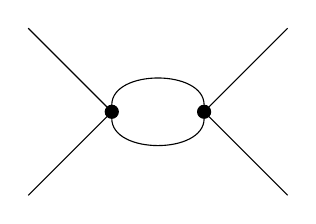
\begin{tikzpicture}[node distance=1cm and 1cm,baseline={([yshift=-.5ex]current bounding box.center)}]
    \coordinate (J1);
    \coordinate[vertex,below right=of J1] (w1);
    \coordinate[below left=of w1] (J2);
    \coordinate[vertex,right=of w1] (w2);
    \coordinate[above right=of w2] (J3);
    \coordinate[below right=of w2] (J4);
    \begin{scope}[every node/.style={scale=.85}]
      \draw (J1) -- (w1);
      \draw (J2) -- (w1);
      \draw (w1) to[in=90,out=90] (w2);
      \draw (w1) to[in=-90,out=-90] (w2);
      \draw (w2) -- (J3);
      \draw (w2) -- (J4);
    \end{scope}
  \end{tikzpicture}
  \quad \Rightarrow \quad
  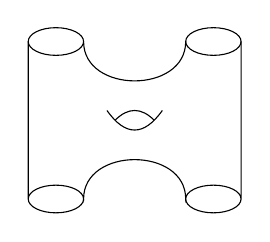
\begin{tikzpicture}[every tqft/.style={draw},baseline={([yshift=-.5ex]current bounding box.center)}]
    \pic[tqft,
      incoming boundary components=2,
      outgoing boundary components=2,
      genus=1,
      every lower boundary component/.style={draw}
    ];
  \end{tikzpicture}
  \quad \cong \quad T^2 \text{ with 4 marked points}.
\end{align*}

In QFT, to obtain the $4$-point correlation function, we summed over
all tree-level, i.e. zero-loop, Feynman diagrams, followed by one-loop
diagrams, etc. Similarly, to obtain the $4$-point scattering amplitude
here, we must sum over all genus zero surfaces with four marked points
and their metrics, then genus one surfaces with four marked points and
their metrics, etc.

Do surfaces of different genus contribute differently to the path
integral? Recall that when we first discussed the gauge symmetries of
the Polyakov action, we found that aside from the already-existing
term, there could only be one other term satisfying all the
gauge symmetries, given by
\[ \chi \coloneqq \frac{1}{4\pi} \int_\Sigma d^2\sigma \, \sqrt{-\gamma} \, R + \frac{1}{2\pi} \int_{\di \Sigma} ds \, k \]
Of course, by Gauss-Bonnet, $\chi$ is nothing more than the {\bf Euler
  characteristic} of the worldsheet. It acts as the {\bf coupling
  constant} for worldsheets of different genus.

\begin{definition}
  An {\bf $n$-string scattering amplitude} involving $n$ strings with
  momenta $(k_i)^\mu$ and states $j_i$ is given by
  \[ S_{j_1 \cdots j_n}(k_1, \ldots, k_n) \coloneqq \sum_{\substack{\text{closed}\\\text{surfaces } \Sigma}} \int \frac{\cD X \, \cD g}{\diff \times \Weyl} \exp(-S_{\text{X}} - \lambda \chi) \prod_{i=1}^n \int d^2\sigma_i \, \sqrt{g(\sigma_i)} \, \cV_{j_i}(k_i, \sigma_i) \]
  where the $\cV_{j_i}$ are the local operators arising from the
  state-operator correspondence. Note that we integrate them over the
  worldsheet to preserve diffeomorphism invariance. Also, since
  $\exp(-\lambda \chi)$ is a topological invariant, it does not depend
  on the {\bf embedding} $X^\mu$ of $\Sigma$ into spacetime, nor the
  metric $g$ on $\Sigma$, so we define $g_s \coloneqq \exp(-\lambda)$,
  the {\bf string coupling constant}, and write
  \[ S_{j_1 \cdots j_n}(k_1, \ldots, k_n) = \sum_{\text{genus } p=0}^\infty g_s^{-(2-2p)} \int \frac{\cD X \, \cD g}{\diff \times \Weyl} \exp(-S_{\text{X}}) \prod_{i=1}^n \int d^2\sigma_i \, \sqrt{g(\sigma_i)} \, \cV_{j_i}(k_i, \sigma_i) \]
\end{definition}

\begin{definition}
  For a fixed genus $p$, let $\Met(\Sigma_p)$ be the space of all
  metrics on any surface $\Sigma_p$ of genus $p$. Then the
  configuration space we are integrating over is
  \[ \frac{\Met(\Sigma_p) \times C^\infty(\Sigma_p, \bR^D) \times (\Sigma_p)^n}{\diff \times \Weyl} \cong \cM(\Sigma_p) \times C^\infty(\Sigma_p, \bR^D) \times (\Sigma_p)^n \]
  where $\cM(\Sigma_p)$ is the {\bf moduli space of genus-$p$ Riemann
    surfaces}. Here, the action of $\Weyl$ on $\Met(\Sigma_p)$ simply
  defines the {\bf conformal classes} $\Conf(\Sigma_p)$ of metrics on
  $\Sigma_p$, i.e. $\Met(\Sigma_p)/\Weyl \cong \Conf(\Sigma_p)$.
\end{definition}

Recall that $\cM(\Sigma_p)$ is actually finite-dimensional, so these
is some hope of ending up with a well-defined integral! There are a
few things we must do in order to have this happen: we must
\begin{enumerate}
\item completely understand the action of $\diff \times \Weyl$ on
  $\Met(\Sigma_p)$ (including the remnant gauge symmetry we
  encountered, in the form of holomorphic diffeomorphisms, even after
  gauge-fixing),
\item use Faddeev-Popov to write $S_{j_1\cdots j_n}(k_1, \ldots, k_n)$
  as a finite-dimensional integral over the moduli space
  $\cM(\Sigma_p)$, and
\item define a measure on $\cM(\Sigma_p)$, hopefully descending from
  $\Met(\Sigma_p)$, so that this integral is well-defined.
\end{enumerate}
Physicists call elements of the moduli space {\bf metric moduli}, or
just {\bf moduli} for short.

\subsection{Integration Measure on the Moduli Space}

We shall begin with items 1 and 3; they are related. But the former is
surprisingly non-trivial for genus $p < 2$. (Usually, people avoid
such difficulties by defining $\cM(\Sigma_p)$ differently for $p < 2$.
But we cannot.)
\begin{enumerate}
\item For genus $p < 2$, there exist {\bf conformal Killing vectors}
  (CKVs) on $\Sigma_p$, i.e. non-trivial transformations in $\diff
  \times \Weyl$ that act as the identity on the metric. We examined
  some, given by holomorphic diffeomorphisms, when we introduced
  gauge-fixing.
\item The CKVs form a group, called the {\bf conformal Killing group}
  $\CKG(\Sigma_p)$. If $\CKG(\Sigma_p)$ has real dimension $k$, then
  we can remove these extra degrees of gauge freedom by fixing $k$
  (real) coordinates of marked points on $\Sigma_p$.
\end{enumerate}
The CKG causes us problems; we must understand how to identify which
infinitesimal $\diff \times \Weyl$ transformations are in the CKG. So
consider an infinitesimal $\diff \times \Weyl$ transformation
\[ \delta g_{ab} = 2\delta \omega g_{ab} - \nabla_a \delta \sigma_b - \nabla_b \delta \sigma_a = (2\delta \omega - \nabla_c \delta \sigma^c)g_{ab} - 2(P_1\delta \sigma)_{ab} \]
where we define a differential operator $P_1$ taking vectors into
traceless symmetric $2$-tensors:
\[ (P_1 \delta \sigma)_{ab} = \frac{1}{2}(\nabla_a \delta \sigma_b + \nabla_b \delta \sigma_a - g_{ab} \nabla_c \delta \sigma^c). \]
By definition, $\delta$ is a CKV iff $\delta g_{ab} = 0$, which, from
the variation $\delta g_{ab}$, happens iff $(P_1\delta\sigma)_{ab} =
0$, called the {\bf conformal Killing equation}. (To get this, just
take the trace of $\delta g_{ab} = 0$, which enforces $2\delta\omega =
\nabla \cdot \delta \sigma$.)

In much the same way, we can identify infinitesimal transformations of
$\Met(\Sigma_p)$ that correspond to moduli: they are variations
$\delta' g_{ab}$ that are {\bf orthogonal} (hang on, we'll define the
metric soon) to all $\diff \times \Weyl$ variations, i.e.
\begin{align*}
  0
  &= \int d^2\sigma \sqrt{g} \, \delta' g_{ab} \left((2\delta \omega - \nabla \cdot \delta \sigma) g^{ab} - 2(P_1 \delta \sigma)^{ab}\right) \\
  &= \int d^2\sigma \sqrt{g} \, \left(\delta' g_{ab} g^{ab}(2\delta \omega - \nabla \cdot \delta \sigma) - 2(P_1^\dag \delta' g)_a \delta \sigma^a\right),
\end{align*}
where we define $(P_1^\dag u)_a = -\nabla^b u_{ab}$. We see from this
calculation that $\delta'$ is a modulus iff
\[ g^{ab}\delta' g_{ab} = 0 \text{ and } (P_1^\dag \delta' g)_a = 0. \]

\begin{exercise}
  Show that in conformal gauge, the conformal Killing equation and the
  condition that $\delta'$ is a modulus become, respectively,
  \[ \di_{\bz} \delta z = \di_z \delta \bz = 0, \quad \di_{\bz} \delta' g_{zz} = \di_z \delta' g_{\bz\bz} = 0, \]
  i.e. CKVs are {\bf holomorphic vector fields} and moduli are {\bf
    holomorphic quadratic differentials}.
\end{exercise}

\begin{definition}
  Define an inner product on symmetric tensors (of any rank) on a
  surface with metric $g$ by
  \[ (A, B)_g \coloneqq \int d^2\sigma \sqrt{g} \, A \cdot B, \]
  where the dot denotes contraction on all indices. Using this inner
  product, define a {\bf metric} $\langle \cdot, \cdot \rangle_{\Met}$
  on $\Met(\Sigma)$ as follows. Fix $g \in \Met(\Sigma)$, and let
  $(g^I)$ be coordinates in an open neighborhood of $g$. Given $X, Y
  \in T_g\Met(\Sigma)$, we can expand them in coordinates as
  \[ X = X^I \pder{}{g^I} = X^I_{a_1b_1} \pder{}{g^I_{a_1b_1}} \in T_g\Met(\Sigma), \quad Y = Y^J \pder{}{g^J} = Y^J_{a_2b_2} \pder{}{g^J_{a_2b_2}} \in T_g\Met(\Sigma). \]
  Then define
  \[ \langle X, Y \rangle_{\Met} \coloneqq (X^I, Y^I)_g = \int_\Sigma d^2\sigma \, \sqrt{g} \, g^{a_1a_2}(\sigma) g^{b_1b_2}(\sigma) X^I_{a_1b_1}(\sigma) Y^I_{a_2b_2}(\sigma). \] 
  Consequently, we get a well-defined measure on $\Met(\Sigma)$.
\end{definition}

\begin{exercise}
  Check that, under this metric, moduli are indeed orthogonal to the
  $\diff \times \Weyl$ action. Indeed, check that we have an {\bf
    orthogonal decomposition} of metric variations
  \[ \delta g = \{\Weyl\} \oplus \{\diff\} \oplus \{\text{moduli}\} = \{\Weyl\} \oplus \im P_1 \oplus \ker P_1^\dag \]
  by showing that $P_1^\dag$ is the adjoint of $P_1$ under $(\cdot,
  \cdot)_{g(x)}$, and recalling that $\ker A^\dag = (\im A)^\perp$ for
  an operator $A$. Also, verify that $\ker P_1$ is the CKG. $P_1$ is
  an important operator!
\end{exercise}

It is fairly easy to check that $\langle \cdot, \cdot \rangle_{\Met}$
is invariant under the $\diff \times \Weyl$ action, so it descends
from $\Met(\Sigma_p)$ to a well-defined metric on $\cM(\Sigma_p)$,
known as the {\bf Weil-Petersson metric}. Hence we also obtain a
well-defined measure on $\cM(\Sigma_p)$.

\subsection{Calculating the Measure Using Faddeev-Popov}

Now we shall apply Faddeev-Popov in order to compute what this measure
on $\cM(\Sigma_p)$ is. Essentially, we shall perform a change of
variables, from integrating over metrics and vertex positions to
integrating over variables corresponding to the orthogonal
decomposition, i.e. integrating over the gauge group, moduli (of
dimension $\tau$), and unfixed vertex positions. In other words, we
wish to find the Jacobian for the transformation
\[ \frac{1}{\diff \times \Weyl}\int_{\Met(\Sigma_p)} \cD g \, d^{2n}\sigma \to \frac{1}{\diff \times \Weyl}\int_{\diff \times \Weyl} \cD \zeta \int_{\cM(\Sigma_p)} d^\tau m \int_{(\Sigma_p)^{n-k/2}} d^{2n-k}\sigma. \]
Note that because of the additional gauge freedom given by the CKG, we
can choose the gauge-fixing conditions now to also fix $\kappa = \dim
\CKG(\Sigma_p)$ of the vertex operator coordinates, so that
$\sigma_i^a \to \hat{\sigma}_i^a$ for some set, denoted $\Fixed$, of
fixed coordinates $(a, i)$.

To find the appropriate Jacobian for this change of variables, we use
Faddeev-Popov. We can directly write down the {\bf Faddeev-Popov
  determinant}:
\[ \Delta_{\text{FP}}(g, \sigma)^{-1} = \int_{\cM(\Sigma)} d^\tau m \int_{\diff \times \Weyl} \cD \zeta \, \delta(\hat{g}(m)^\zeta - g) \prod_{(a, i) \in \Fixed} \delta((\hat{\sigma}_i^\zeta)^a - \sigma_i^a). \]
Previously, we rewrote the right hand side as an integration over
infinitesimal transformations under the false assumption that the
gauge group acted freely on the configuration space of embeddings and
metrics. This was OK because we did not explicitly compute anything
that depended on getting factors correct in numerical results.
However, now we care. Note that:
\begin{enumerate}
\item an integral over infinitesimal transformations, i.e. the Lie
  algebra, only captures behavior in the connected component of the
  identity in $\diff \times \Weyl$;
\item by homogeneity, the value of the integral in the connected
  component of the identity is the same as the value in any other
  connected component;
\item after removing the CKG, the action of the connected component of
  the identity $(\diff \times \Weyl)_0 = \diff_0 \times \Weyl$ is free.
\end{enumerate}
Hence we can, again, write the integral as an integral over the Lie
algebra, but now we have a constant, finite factor $n_R$ in front:
\[ \Delta_{\text{FP}}(\hat{g}, \sigma)^{-1} = n_R \int d^\tau (\delta m) \, \cD(\delta \omega) \, \cD(\delta \sigma) \, \delta(\delta g_{ab}) \prod_{(a,i) \in \Fixed} \delta(\delta \sigma^a(\hat{\sigma}_i)), \]
where $n_R$ is the size of the {\bf mapping class group} $\Mod(\Sigma)
= |\diff/\diff_0|$. (We don't care about $\Weyl$, since it is
trivially connected.)

Now we follow the exact same procedure as we did for inverting the
Faddeev-Popov determinant for the Polyakov action: compute $\delta
g_{ab}$, introduce auxiliary variables of integration $x$ and
$\beta_{ab}$ to write the delta functionals as exponentials, integrate
out $\delta \omega$ to obtain the constraint that $\beta_{ab}$ is
traceless, and replace the bosonic variables $(\delta \sigma^a,
\beta_{ab}, x_{ai}, \delta m^t)$ with fermionic variables $(c^a,
b_{ab}, \eta_{ai}, \zeta^t)$, to get
\[ \Delta_{\text{FP}}(\hat{g}, \sigma) = \frac{1}{n_R} \int \cD b \, \cD c \, d^\tau \zeta \, d^\kappa \eta \, \exp\left(-\frac{1}{4\pi} (b, 2P_1 c - \zeta^j \di_j \hat{g})_{\hat{g}} + \sum_{(a,i) \in \Fixed} \eta_{ai} c^a(\hat{\sigma}_i)\right). \]
(We've added in some convenient normalization factors.) Finally, we do
the integratation over the Grassmann parameters $\eta_{ai}$ and
$\zeta^i$. The (somewhat elegant) result is
\[ \Delta_{\text{FP}}(\hat{g}, \sigma) = \frac{1}{n_R} \int \cD b \, \cD c \, \exp(-S_{\text{G}}) \prod_{j=1}^\tau \frac{(b, \di_j \hat{g})_{\hat{g}}}{4\pi} \prod_{(a,i) \in \Fixed} c^a(\hat{\sigma}_i) \]

But there is a nicer way to write $\Delta_{\text{FP}}$. As a Jacobian,
it is a determinant, and as a Jacobian for a change of variables into
an orthogonal decomposition, we expect it to decompose as a product of
determinants. Indeed, it does. First, obtain real eigenbases
$\{\cC_J\}$ and $\{\cB_K\}$ for the operators $P_1^\dag P_1$ and $P_1
P_1^\dag$, i.e.
\[ P_1^\dag P_1 (\cC_J)^a = v_J^2 (\cC_J)^a, \quad P_1 P_1^\dag (\cB_K)_{ab} = w_K^2 (\cB_K)_{ab}, \]
normalized such that $(\cC_J, \cC_{J'}) = \delta_{JJ'}$ and $(\cB_K,
\cB_{K'}) = \delta_{KK'}$. These eigenbases are related. Note that
$P_1\cC_J$ is an eigenfunction of $P_1P_1^\dag$, and similarly,
$P_1\cB_K$ is an eigenfunction of $P_1^\dag P_1$. Hence there is a
one-to-one correspondence between the eigenbases $\{\cC_J\}$ and
$\{\cB_K\}$ except for when $P_1\cC_J = 0$ or $P_1\cB_K = 0$, i.e.
when the eigenfunction has a zero eigenvalue. The $\cC_J$ with zero
eigenvalue correspond to $\kappa$ CKVs, and the $\cB_K$ with zero
eigenvalue correspond to $\tau$ moduli. Denote these eigenfunctions of
zero eigenvalue $\{(\cC_{0j})^a\}_{j=1}^\kappa$ and
$\{(\cB_{0k})_{ab}\}_{k=1}^\tau$. The rest (of non-zero eigenvalue)
are indexed as normal with $J, K = 1, \ldots$, and satisfy
$(\cB_J)_{ab} = (1/w_J)(P_1 \cC_J)_{ab}$.

If we rewrite the integral for $\Delta_{\text{FP}}$ in terms of these
eigenbases, we get
\begin{align*}
  \Delta_{\text{FP}} = \int &\prod_{k=1}^\tau db_{0k} \prod_{j=1}^\kappa dc_{0j} \prod_J db_J \, dc_J \, \exp\left(-\frac{w_J b_J c_J}{2\pi}\right) \\
  &\quad \times \left(\prod_{k'=1}^\tau \sum_{k''=1}^\tau \frac{b_{0k''}}{4\pi} (\cB_{0k''}, \di_{k'}\hat{g})\right) \left(\prod_{(a,i) \in \Fixed} \sum_{j'=1}^\kappa c_{0j'} (\cC_{0j'})^a(\sigma_i)\right),
\end{align*}
which is just a product of three Gaussian integrals. Recalling how to
do Gaussian integrals with insertions, i.e. of the form $\int dx \,
\exp(-x^2) x^k$, we get
\[ \Delta_{\text{FP}} = \left[\det\left(\frac{(\cB_{0k}, \di_{k'}\hat{g})}{4\pi}\right)_{k,k'=1}^\tau\right]\left[\det\left((\cC_{0j})^a(\sigma_i)\right)_{j=1, (a,i) \in \Fixed}^\kappa\right] \left[\det\nolimits' \left(\frac{P_1^\dag P_1}{2\pi}\right)^{1/2}\right], \]
where $\det'$ indicates that we omit zero eigenvalues. Otherwise the
whole expression is trivially zero.

For tree-level and one-loop amplitudes, evaluating this expression for
$\Delta_{\text{FP}}$ is not too bad. For higher-loop amplitudes, there
is more work involved. But in that case we must put in more work
anyway: to even integrate on the moduli space requires us to put {\bf
  Fenchel-Nielsen} coordinates on it, which is not an easy task.

\subsection{The $X^\mu$ Integration}

It remains to handle the $X^\mu$ integration
\[ \left\langle \prod_{i=1}^n \int d^2\sigma_i \, \sqrt{g(\sigma_i)} \, \cV_{j_i}(k_i, \sigma_i) \right\rangle \coloneqq \int \cD X \, \exp(-S_X) \prod_{i=1}^n \int d^2\sigma_i \, \sqrt{g(\sigma_i)} \, \cV_{j_i}(k_i, \sigma_i). \]
To evaluate this integral, we use the same trick we used in QFT:
introduce a formal variable $J$, write down the {\bf generating
  functional}
\[ Z[J] = \left\langle \exp\left(i\int d^2\sigma \, J_\mu X^\mu\right) \right\rangle \]
and do tricks with $J^\mu(\sigma)$ in order to get the vertex operator
insertions we want. We can directly compute $Z[J]$ by writing the
Polyakov action as
\[ S_X = \frac{T_0}{2} \int d^2\sigma \, X_\mu \Delta_g X^\mu, \quad \Delta_g \coloneqq \nabla^2 = \frac{1}{\sqrt{g}} \di_a \sqrt{g} \, g^{ab} \di_b, \]
which is a Gaussian. Expand $X$ and $J$ in terms of an eigenbasis of
the Laplacian:
\[ \Delta_g \cX_I = -\omega_I^2 \cX_I, \quad X^\mu = \sum_I x_I^\mu \cX_I, \quad J^\mu = \sum_I J_I^\mu \cX_I, \]
where the eigenfunctions $\psi_I$ are chosen to be orthogonal with
respect to $(\cdot, \cdot)_g$. Then
\[ Z[J] = \prod_{I,\mu} \int \cD X^\mu \, \exp\left(-\frac{T_0}{2} \omega_I^2 x_I \cdot x_I + iJ_I \cdot x_I\right). \]
Before doing the Gaussian integrals, note that the zero mode $\cX_0$
is special: since $\nabla^2 \cX_0 = 0$, it has an extremum in the
interior of the Riemann surface $\Sigma$. By the maximum modulus
principle, $\cX_0$ must be constant. Hence its corresponding Gaussian
integral becomes $\int \cD X^\mu \exp(iJ_0 \cdot x_0) =
\delta^D(J_0)$.

\begin{exercise}
  Review how to do Gaussian integrals, in particular the $Z[J]$
  integral from QFT, and calculate that
  \[ Z[J] = i(2\pi)^D \delta^D(J_0) \det\nolimits' \left(\frac{T_0}{\pi}\Delta_g\right)^{-d/2} \exp\left(-\frac{1}{2} \int d^2 \sigma_1 \, d^2\sigma_2 \, J(\sigma_1) G'(\sigma_1, \sigma_2) J(\sigma_2)\right), \]
  where the {\bf Green's function} (excluding zero modes) is
  \[ G'(\sigma_1, \sigma_2) \coloneqq \sum_{I \neq 0} \frac{1}{T_0} \frac{1}{\omega_I^2} \cX_I(\sigma_1) \cX_I(\sigma_2). \]
  Verify that $G'(\sigma_1, \sigma_2)$ satisfies
  \[ -T_0 \Delta_g G'(\sigma_1, \sigma_2) = \sum_{I \neq 0} \cX_I(\sigma_1) \cX_I(\sigma_2) = \frac{1}{\sqrt{g}} \delta^2(\sigma_1 - \sigma_2) - \cX_0^2 \]
  using the completeness relation for the eigenbasis $\{\cX_I\}$.
\end{exercise}

We shall use this differential equation for the Green's function in
order find out what it is. Note that it depends on $\Delta_g$, which
changes with different moduli, and, in particular, different genus.
Hence for every $n$, to compute the $n$-loop corrections to the
amplitude, we need to find $G'$ for every element in the moduli space.

\section{Tree-Level Amplitudes}

In this section, we compute tree-level amplitudes for {\bf $n$-tachyon
  scattering}, which, for closed strings, corresponds to $\Sigma =
S^2$ with $n$ marked points with {\bf tachyon vertex operators}
$\cV_{j_i}(k_i, \sigma_i) = \NO{e^{ik\cdot X}}$. Hence we must first
understand $\cM(S^2)$ and $\CKG(S^2)$.

\begin{proposition}
  $\cM(S^2)$ is a single point, and $\CKG(S^2) \cong \PSL(2, \bC)$,
  with real dimension $6$.
\end{proposition}

\begin{proof}
  Take the standard atlas for $S^2$ given by stereographic projection:
  one coordinate $z$ on $S^2 \setminus \{N\}$, i.e. everywhere except
  the north pole, and another coordinate $u$ on $S^2 \setminus \{S\}$,
  i.e. everywhere except the south pole. In conformal gauge, we know
  from a previous exercise that moduli are holomorphic quadratic
  differentials $\delta g_{zz}(z)$ and CKVs are holomorphic vector
  fields $\delta z(z)$. But these objects must be well-defined
  globally, so we need to consider them on the $u$ patch:
  \[ \delta u = \pder{u}{z} \delta z = -z^{-2} \delta z, \quad \delta g_{uu} = \left(\pder{u}{z}\right)^{-2} \delta g_{zz} = z^4 \delta g_{zz}. \]
  If $\delta g_{uu}$ is well-defined at $u = 0$, i.e. the north pole,
  then $\delta g_{zz} \propto z^{-4}$ as $|z| \to \infty$. Hence
  $\delta g_{zz}$ is a bounded entire function, which, by Liouville's
  theorem, is constant. In the moduli space, we have already modded
  out by Weyl transformations, so all constant functions are
  equivalent. (In fact, by the uniformization theorem, every metric is
  equivalent to the constant-curvature metric induced by the inclusion
  $S^2 \to \bR^3$.) However, for CKVs, we only need $\delta z \propto
  z^2$ as $|z| \to \infty$, so in general,
  \[ \delta z = a_0 + a_1z + a_2z^2, \quad \delta \bz = a_0^* + a_1^*\bz + a_2^*\bz^2. \]
  Hence $\dim_{\bR} \CKG(S^2) = 6$. It is well-known that these are
  precisely the infinitesimal transformations of the M\"obius group
  \[ \PSL(2, \bC) = \left\{\frac{az+b}{cz+d} : ad - bc = 1\right\}/((a, b, c, d) \sim (-a, -b, -c, -d)). \qedhere \]
\end{proof}

We first compute the $X^\mu$ integral using the results of the
previous section. Using the fact that $\di \bdi \ln |z| = 2\pi
\delta(z)$, by solving the DE, we get the Green's function
\[ G'(\sigma_1, \sigma_2) = -\frac{1}{4\pi T_0} \ln |z_1 - z_2|^2 + f(z_1, \bz_1) + f(z_2, \bz_2), \quad f(z, \bz) \coloneqq \frac{\cX_0^2}{8\pi T_0} \int d^2 w \, e^{2\omega(z,\bz)} \ln |z - w|^2 + C \]
where the function $f$ acts as a {\bf regulator} that cancels out in
the final amplitudes, and $C$ is just a constant to make sure $G'$ is
orthogonal to $\cX_0$, a constant. The tachyon vertex operators
$\NO{e^{ik_i\cdot X}}$ correspond to $J(\sigma) = \sum_i \delta(\sigma
- \sigma_i)$. Consequently,
\[ Z[J] = C_{S^2}^{\text{X}} \delta^D(\sum_i k_i) \exp\left(-\sum_{i < j} k_i \cdot k_j G'(\sigma_i, \sigma_j) - \frac{1}{2}\sum_i k_i^2 G'_r(\sigma_i, \sigma_i)\right), \; C_{S^2}^{\text{X}} \coloneqq \frac{i(2\pi)^D}{\cX_0^D} \det\nolimits' \left(\frac{T_0}{\pi}\Delta_g\right)^{-\frac{D}{2}}, \]
where the $G'_r \neq G'$ because of the normal ordering. In fact, for
normal-ordered vertex operators, we get $G'_r(\sigma, \sigma) = 2f(z,
\bz)$, so
\[ Z[J] = C_{S^2}^{\text{X}} \delta^D\left(\sum_i k_i\right) \prod_{i<j} |z_i - z_j|^{k_i \cdot k_j/2\pi T_0}. \]
Note that the regulator $f$ has canceled. 

Since the sphere has no moduli, we are free to ignore the integral
over moduli space. Most of the Faddeev-Popov measure becomes constant,
except the Jacobian for the CKG. From
our computation of the CKG, we know a basis for CKVs is given by
$\cC^z = 1, z, z^2$ and $\cC^{\bz} = 1, \bz, \bz^2$, so
\[ \Delta_{\text{FP}} = C_{S^2}^{\text{G}} \det(\cC^a_{0j}(\sigma_i)) = C_{S^2}^{\text{G}} \det((z_i)^{j-1})_{i,j=1}^3 \det((\bz_i)^{j-1})_{i,j=1}^3 = C_{S^2}^{\text{G}} |z_1 - z_2|^2 |z_1 - z_3|^2 |z_2 - z_3|^2, \]
absorbing the two other (now constant) determinants in
$C_{S^2}^{\text{G}}$. Assume that we are scattering $n > 2$ tachyons,
so that the $\dim_{\bC} \CKG(S^2) = 3$ degrees of freedom can fix the
positions $\hat{z}_1, \hat{z}_2, \hat{z}_3$ of the first three local
operators: it is well-known that the M\"obius transformations $\PSL(2,
\bC)$ act transitively on triplets of points, i.e. is $3$-transitive.

\begin{proposition}
  The closed string, tree-level, $n$-tachyon scattering amplitude is
  given by
  \[ S_{j_1 \cdots j_n}(k_1, \ldots, k_n) = g_s^{-2+n} C_{S^2}^{\text{X}} C_{S^2}^{\text{G}} \delta^D\left(\sum_{i=1}^n k_i\right) |\hat{z}_1 - \hat{z}_2|^2 |\hat{z}_1 - \hat{z}_3|^2 |\hat{z}_2 - \hat{z}_3|^2 \int \prod_{i=4}^n d^2 z_i \prod_{i<j} |z_i - z_j|^{k_i \cdot k_j/2\pi T_0} \]
  for any choice of $\hat{z}_1, \hat{z}_2, \hat{z}_3 \in \bC^2$.
\end{proposition}

The closed string, four-tachyon scattering amplitude is the first
computed non-trivial string scattering amplitude, and therefore has a
name: the {\bf Virasoro-Shapiro amplitude}. We shall compute it
explicitly.

\begin{example}[Virasoro-Shapiro amplitude]
  Write $\alpha' = 1/2\pi T_0$. Pick $\hat{z}_1 = 1$, $\hat{z}_2 = 0$,
  and $\hat{z}_3 = \infty$. Then any term $|\hat{z}_3 - z_i|$ can be
  treated as $|\hat{z}_3|$, so
  \[ |\hat{z}_1 - \hat{z}_3|^{2+\alpha' k_1\cdot k_3}|\hat{z}_2 - \hat{z}_3|^{2+\alpha' k_2 \cdot k_3}|\hat{z}_3 - z_4|^{\alpha' k_3 \cdot k_4} = |\hat{z}_3|^{4 + \alpha' k_3 \cdot (k_1 + k_2 + k_4)} = |\hat{z}_3|^0 = 1, \]
  by recalling that on-shell tachyons satisfy $k^2 = 4/\alpha'$, and
  therefore, using momentum conservation,
  \[ 4 + \alpha' k_3(k_1 + k_2 + k_4) = 4 - \alpha' k_3^2 = 4 - 4 = 0. \]
  Introduce {\bf Mandelstam variables} like we did for $4$-point
  scattering in QFT:
  \[ s \coloneqq -(k_1 + k_2)^2, \quad t \coloneqq -(k_1 + k_3)^2, \quad u \coloneqq -(k_1 + k_4)^2, \]
  which satisfy $s + t + u = -16/\alpha'$. Again using the on-shell
  condition and momentum conservation, we can show that the remaining
  part of the integral is
  \[ \int d^2z_4 \, |1 - z_4|^{\alpha' k_1 \cdot k_4} |z_4|^{\alpha' k_2 \cdot k_4} = \int d^2z_4 |1 - z_4|^{-(\alpha' u)/2 - 4} |z_4|^{-(\alpha' t)/2 - 4}. \]
  Now recall that using the {\bf Euler beta function},
  \[ \int d^2z \, |z|^{2a-2} |1-z|^{2b-2} = 2\pi \frac{\Gamma(a) \Gamma(b) \Gamma(c)}{\Gamma(a+b) \Gamma(a+c) \Gamma(b+c)}, \quad a + b + c = 1, \]
  so that our final expression is
  \[ S_{j_1 \cdots j_4}(k_1, \ldots, k_4) = g_s^2 C_{S^2}^{\text{X}} C_{S^2}^{\text{G}} \delta^D(k_1 + \cdots + k_4) 2\pi \frac{\Gamma(-1 - \frac{\alpha'}{4} s)\Gamma(-1 - \frac{\alpha'}{4} t)\Gamma(-1 - \frac{\alpha'}{4} u)}{\Gamma(2 + \frac{\alpha'}{4}s)\Gamma(2 + \frac{\alpha'}{4}t)\Gamma(2 + \frac{\alpha'}{4}u)}. \]
\end{example}

The analogous amplitude for open strings, called the {\bf Veneziano
  amplitude}, led to the birth of string theory in the 1970s.

\section{One-Loop Amplitudes}

In this section, we compute one-loop corrections to amplitudes for
$n$-tachyon scattering, which, for closed strings, corresponds to
$\Sigma = T^2$, the torus, with $n$ marked points. Hence we must
understand $\cM(T^2)$ and $\CKG(T^2)$. Recall that $\bH^2$ is the {\bf
  hyperbolic plane}, which can be identified with the {\bf upper half
  plane}.

\begin{proposition}
  $\cM(T^2) = \bH^2/\PSL(2, \bZ)$, and $\CKG(T^2) = U(1) \times U(1)$.
\end{proposition}

\section{Higher-Order Amplitudes}

\end{document}
